\documentclass[12pt, a4paper, oneside]{book}
\usepackage[left=3.0cm, top=3.0cm, right=2.5cm, bottom=3.0cm]{geometry}
\usepackage[utf8]{inputenc}
\usepackage[T1]{fontenc}
\usepackage[english,hungarian]{babel}
\selectlanguage{hungarian}
\usepackage{fancyhdr}
\usepackage{setspace}
\usepackage{listings}
\usepackage{makeidx}
\usepackage{natbib}
\usepackage{url}
\usepackage{color}
\usepackage[usenames,dvipsnames]{xcolor}
\usepackage{graphicx}
\makeindex

\newenvironment{abstract}
{\newpage \pagestyle{empty} \vspace*{\fill} \begin{center}\em{Kivonat}\end{center}}
{\vspace*{\fill} \newpage}

\definecolor{light-gray}{gray}{0.6}
\lstnewenvironment{code}[2]
{\lstset{basicstyle=\footnotesize, showstringspaces=false, emphstyle=\textbf,
caption=#2, language= #1, frame=single, xleftmargin=1.5cm, xrightmargin=1.5cm,
rulecolor=\color{light-gray}, belowskip=0.75cm, aboveskip=0.5cm,
framexleftmargin=0.5cm, framexrightmargin=0.5cm}}
{}

\pagestyle{fancy}
\renewcommand{\chaptermark}[1]{%
\markboth{\thechapter.%
\ \chaptername.\ #1}{}}

\fancyhead[L]{}

\renewcommand\lstlistingname{}
%\renewcommand\lstlistlistingname{Ábrák}
\lstset{caption=\thelstlisting. \lstlistingname}

\author{Czinkos Zsolt}
\title{Erlang/OTP: magas rendelkezésre állású, elosztott rendszerek fejlesztése}
\date{2012-04-28}

\renewcommand{\maketitle}{
\begin{titlepage}
\noindent Budapesti Corvinus Egyetem\\
Gazdálkodástudományi Kar\\
Levelező Tagozat\\

\vspace{6cm}

\begin{center}
\Large{Erlang/OTP}\\
\vspace{0.3cm}
\large{Magas rendelkezésre állású, elosztott rendszerek
fejlesztése}
\end{center}

\vfill

\begin{flushright}
Készítette: Czinkos Zsolt\\
Gazdaságinformatikus (BSc) Szak\\
2012\\
\end{flushright}

\vspace{0.5cm}

\begin{center}
Konzulens: Dr. Fodor Szabina
\end{center}

\end{titlepage}
}

\begin{document}
\maketitle

\onehalfspacing

\begin{abstract}
Az Erlang programozási nyelvet az Ericssonnál hozták létre hálózati
eszközök, telefonrendszerek programozására. A magas telekom elvárások
tükröződnek az Erlangban fejlesztett rendszerek architektúrájában,
amely az Open Telecom Platform szoftverkönyvtárban ölt testet. A dolgozat
bemutatja az Erlang programozási nyelvet, a fejlesztési elveket és
alkalmazási lehetőségét a webes technológiára épülő alkalmazások területén.
\end{abstract}

\newpage
\pagestyle{empty}
\vspace*{\fill} 
\hfill \emph{anyukámnak}
\vspace*{\fill} 
\newpage

\pagestyle{fancy}

\tableofcontents

\chapter{Bevezetés}

Az Internet -- azon belül különösen a Web -- terjedésével párhuzamosan nőtt az
igény kiszámítható, jó minőségű szolgáltatásokra. A szolgáltatóknak egyre
magasabb elvárásoknak kell megfelelniük -- nem utolsó sorban azért, mert a
felhasználók fejében a web és az ingyenes tartalom összeforrt. Még színvonalas
termékekért is nehezen adnak ki pénzt, nemhogy hibás, elavult tartalomért,
akadozó és kiszámíthatatlanul működő szolgáltatásokért. Ma már a hálózat nem
csupán mérnököknek, kutatóknak érdekes kábelezést jelent, amely így-úgy hasznos
tudományos kutatásaik során, hanem a mindennapi élet részét képező társadalmi
kapcsolatok \textit{reprezentációját} is. A felhasználó egyre aktívabb
\textit{cselekvője} ezeknek a valós vagy virtuális világban létrejött
hálózatoknak, egyre inkább itt keresi (és többnyire találja meg) azt a teret,
ahol ismerik, és ő is ismer; ahol ura annak az eszköztárnak, amelynek
birtokában különböző (rövid, prompt, aszinkron, szöveg, hang vagy videó)
\textit{üzenetek} segítségével ápolni tudja kapcsolatait. Ez a
kapcsolatrendszer és eszköztár jelenti azt az új mikrokozmoszt, amelyben a
felhasználó -- cselekvő- és befolyásolóképessége tudatában -- kényelemben és
biztonságban érzi magát.

Ez a kényelem és biztonság \textit{függővé} tesz: világunk megszokott
működésének zavarait nehezen vagy egyáltalán nem tudjuk tolerálni,
kiszolgáltatottnak és tehetetlennek érezzük magunkat. Ilyenkor derül ki, hogy
bár mikrokozmoszunkat ismerni véljük, az azt működtető rendszer elemeit meg sem
tudjuk nevezni, csak azt tudjuk, hogy \glqq{}van\textquotedblright{} (ez a
valami pillanatnyilag a legtöbb ember számára néhány cég szolgáltatásában ölt
testet: Facebook, Google, Twitter). A szoftverfejlesztőknek, tervezőknek e
világ működtetéséhez szükséges rendszert kell tudniuk megépíteni és
üzemeltetni úgy, hogy a felhasználók a lehető legkevesebb alkalommal
szembesüljenek azzal, hogy kihúzták alóluk a talajt. Nem emberbaráti, hanem
üzleti megfontolások miatt.

A weben a sikerhez elengedhetetlen a folyamatos és megbízható szolgáltatás,
nagyon alacsony az ingerküszöb, ha egy oldal betöltődése tovább tart 4
másodpercnél, már odébb is állt a felhasználó.  Ha túl sokszor kap hibaüzenetet --
amitől jobb esetben ingerült lesz, rosszabb esetben halálra rémül, hátha ő
rontott el valamit --, keres mást \citep{AkamaiReport}.  Éppen ezért nagyon
fontos, hogy olyan rendszert építsünk,

\begin{enumerate} 
  \item amely folyamatosan, megszakítás nélkül működik;
  \item amely megfelelő válaszidővel, sebességgel működik;
  \item amely funkcionálisan jól működik;
  \item amelyben a felmerülő hibák nyomon követhetők, kezelhetők.
\end{enumerate}

A fentebb már említett vezető webes cégek mind megfelelnek ezeknek a
követelményeknek, persze nem kevés munka és pénz árán. A felhasználót azonban a
legkevésbé sem érdekli, hogy a szolgáltatást nyújtó üzleti vállalkozás hogyan
tudja működtetni rendszerét, hány embert alkalmaz stb. Őt az érdekli, hogy
neki ingyen vagy elérhető áron a lehető legtöbbet nyújtsa. Ez az elvárása
sajnos (vagy szerencsére) nem csak a mamutcégekkel szemben áll fent, hanem
minden webes céggel szemben, mindenhol szeretné megkapni azt a minőséget,
amihez hozzászokott. Azt a céget tekinti profinak, jónak, ami ugyanazt tudja
nyújtani. Ha egy cég sikert akar, akkor már induláskor fel kell készülnie arra,
hogy ha elsül a kapanyél, és özönlenek a felhasználók, akkor tartani tudja az
iramot, ki tudja szolgálni ugrásszerűen megnőtt ügyfélkörét; miközben egy kezdő
vállalkozás nem engedhet meg magának földrajzilag diverzifikált több tízezer
gépes szerverparkot: kicsiből indulva kell képesnek lennie a növekedésre.

Hogyan lehet olyan rendszert építeni, amellyel neki lehet vágni egy webes
vállalkozásnak úgy, hogy ne kelljen attól félni, mi lesz, ha holnap regisztrál
még 10 ezer felhasználó (4 másodperc!), vagy ha tönkremegy az egyik gép?

Számos programozási nyelv és környezet közül lehet ma már választani, amely
alkalmas erre a feladatra, ez a dolgozat az Erlang programozási nyelvet és a
hozzá kapcsolódó Open Telecom Platform-ot (OTP) mutatja be. Az Erlang egy
funkcionális programozási nyelv, amelyet az Ericsson fejlesztett ki mintegy 20
évvel ezelőtt telefonrendszerek, szoftveres kapcsolóközpontok programozásához,
a telekommunikációs iparban szokásos rendkívül magas elvárásoknak megfelelően
\citep{ArmstrongBook}. 

Az Erlang megalkotásánál az elsődleges cél magas rendelkezésre állású
(\emph{highly available}), hibatűrő (\emph{fault tolerant}) redundáns
rendszerek építése volt. Ez az, amire az Erlang igazán alkalmas, ez az a
terület, ahol az Erlangnak évtizedes múltja van: akár 99,999\%-os
rendelkezésre állás biztosításában. Ez hozzávetőleg 5 perc kiesés
évente. Az Ericsson AXD nevű terméke ennél magasabb rendelkezésre állást is
elért: 99.9999999\%-ot \citep{CesariniBook}.

1998-ban \emph{open source}-szá vált a nyelv és a platformot adó
szoftverkönyvtárak, azóta bárki használhatja bármilyen feladatra, számos
önkéntes és cég teszi be a közösbe a maga alkalmazását: HTTP szervert, NoSQL
adatbáziskezelőt, szakdolgozatot.

\newpage

\chapter{Elméleti alapok} 

Az Erlang nyelvet rendkívül magas rendelkezésre állású, elosztott rendszerek
készítéséhez hozták létre. Nem akadémiai környezetben született, a legfőbb cél
az volt, hogy profitot termeljenek a segítségével: a szoftverek hamarabb
készüljenek el; a megrendelő azt kapja, amit szeretett volna; a termékek
karbantarthatóak legyenek; redundáns, elosztott környezetben működjenek
(folyamatosan); kapacitásuk növelhető legyen. A vezérelv az volt, hogy ,,minden
szoftver hibás'', mindig előfordul olyan hiba, amelyet nem kellő
körültekintéssel, nem megfelelő specifikáció birtokában megírt szoftver okoz.
Nem lehet úgy tenni, mintha egy szoftver valaha is ,,készen'' lenne, és utána már
nem kellene javítani, új igényeknek megfelelően bővíteni (újabb hibákat
elkövetni). Azt is figyelembe kellett venni, hogy a magas
rendelkezésre állás megkövetelte redundáns architektúra párhuzamos programozást
igényel, nem egy processzoron kell futni, hanem többön, sőt több gépen. Az
Erlang egyik megalkotója, Joe Armstrong, az itt leírt elvekre, módszerekre a
\emph{concurrency-oriented programming} kifejezést használta
\citep{ArmstrongBook}.

Az Erlang lényegében egy magas szintű nyelv konkurens rendszerek
fejlesztéséhez. A párhuzamos programozás komplex feladatok esetében sokkal
képzettebb, tapasztaltabb (így drágább) fejlesztőket kíván meg, egyáltalán nem
kicsi a lépés a nem párhuzamos pogramozástól (\emph{sequential programming}).
Egyszerűen fogalmazva: egynél több cselekvő dolgozik egyazon rendszeren belül,
ezért az egyes állapotváltoztatásoknál gondoskodni kell arról, hogy a több
helyről kezdeményezett műveletek után a rendszer állapota konzisztens maradjon.

A Java nyelvben például a párhuzamos programozást a \emph{thread}-ek teszik
lehetővé, a konzisztens állapot megőrzését pedig a \emph{synchronized}
kulcsszóval jelölt metódusokkal, programblokkokkal lehet elérni. Az Erlanggal
más utat választottak, két alapra építettek: a \emph{funkcionális
programozásra} és az \emph{aktor modellre}.
 
\section{Funkcionális programozás} 

Az Erlang funkcionális programozási nyelv. Az imperatív nyelvekkel szemben,
ahol egy implicit állapot (\emph{state}) változik adott nyelvi konstrukciók
eredményeképp, a tisztán funkcionális nyelvekben nincs implicit állapot, a
függvények mellékhatás-mentesek (\emph{side-effect free}). Minden függvényhívás
tartalmaz minden szükséges argumentumot, ami az eredményhez szükséges (akár
explicit állapotot is, ha szükséges), és az azonos paraméterekkel rendelkező
függvényhívások mindig ugyanazt az eredményt adják (\emph{referential
transparency}). Egyszerű matematikai példával élve: az \texttt{f(x) = x + 1}
függvény azonos x értékekre mindig azonos eredményt ad.

A széles körben elterjedt imperatív nyelvekben (Java, C) az állapot
változtatására szolgáló, a vezérlést végző nyelvi elemek egymásutáni
használatával lehet leírni a működés ,,hogyanját''. Változók értékadása,
feltételes elágazások, ciklusok adják a működés logikáját: mit mi után milyen
feltételek teljesülése esetén kell végrehajtani \citep{Hudak}. Például a Fibonacci-sor Java
megvalósítása:

\begin{code}{java}{Fibonacci -- Java}
int a=0, b=1;
public static int fib(int n) {
  for(int i=0; i<n; i++) {
    int c = a;
    a = b;
    b = c + b;
  }
  return a;
}
\end{code}

A fenti egyszerű példában szerepel értékadás, feltétel vizsgálat és ciklus is.
A végrehajtás során az \texttt{a} változó többször kap új értéket, a ciklus futásának
végén tartalmazza az eredményt.

Az Erlang deklaratív nyelv, a ,,hogyan'' helyett a ,,mit'' írja le: a fejlesztő
kifejezéseket ad meg mintaillesztésekkel -- kijelentéseket tesz. Funkcionális
nyelveknél a függvény alapvető nyelvi elem, amelynek segítségével a működés
leírható. A Fibonacci példa Erlang változata:

\begin{code}{erlang}{Fibonacci -- Erlang}
fib(0) -> 0; 
fib(1) -> 1; 
fib(N) when N > 0 -> fib(N-1) + fib(N-2).  
\end{code} 

Ebben az esetben a fib függvény deklarációja három állítás
(\emph{function clause}): melyik argumentum esetén mit kell tenni. Az imperatív
nyelvekben megszokott struktúrák helyett más megoldásokkal kell élni. Ciklus
helyett rekurzív függvényhívásokkal, feltételes elágazás helyett a függvény
deklarációba írt kifejezéssel (jelen esetben pozitív számokra értelmezett a
függvény).

A funkcionális pogramnyelvek fontos ismérve az is, hogy a függvények teljes jogú
elemei a nyelvnek (\emph{first class functions}). Bárhol, ahol valamilyen érték
szerepelhet, függvény is: listák, rekordok, adatszerkezetek elemeként. Függvény
argumentuma illetve visszatérési értéke is lehet függvény (\emph{higher order
functions}). Például egy lista elemeit többféle szempont szeretnénk szűrni.
Először a páros számokat, majd utána a páratlanokat:

\begin{code}{erlang}{}
Paros = fun(N) when N rem 2 == 0 -> true;
           (_)                   -> false.

Paratlan = fun(N) when N rem 2 == 1 -> true;
              (_)                   -> false.


Lista = [1, 2, 3, 4, 5, 6, 7, 8, 9].
ParosSzamok = lists:filter(Paros, Lista).
ParatlanSzamok = lists:filter(Paratlan, Lista).
\end{code}

A \texttt{lists:filter} függvény a megadott lista minden elemére lefuttatja a
\texttt{Paros} vagy a \texttt{Paratlan} függvényt, és ha igaz értéket kap
vissza, akkor bennehagyja a listában a vizsgált elemet. A \texttt{Paros}
illetve \texttt{Paratlan} függvények változók (amik nem igazi változók, csak
egyszer kaphatnak értéket), amelyek értéke egy-egy névtelen függvény
(\emph{$\lambda$ function}).

Az Erlang nem tisztán funkcionális környezet. Mivel ipari alkalmazásra készült,
lehet írni olyan függvényeket, amelyek nem mellékhatás-mentesek, például fájl-
és adatbázis műveletek. A funkcionális programozás alapelvei azonban jelen
vannak, lehet tisztán funkcionális alkalmazást is írni, és a fentebb
ismertetett elvek maradéktalanul alkalmazhatók. Nem léteznek globális változók,
amelyek értékét több függvényből is módosítani lehetne, minden változó
(pontosabban értékadás egy névhez) csak az adott függvényen belül értelmezett,
a szükséges állapotot a függvény argumentumai közt explicit kell megadni, és a
visszatérési értékbe is betenni. A párhuzamos programozást ez nagyban
megkönnyíti: nem kell attól félni, hogy egy értéket egy másik folyamat vagy
függvényhívás felülír, mindig minden ,,kézben van'' \citep{ArmstrongThesis}.
Hogyan lehet így bármi használhatót írni? Hogyan lehet egy komplex rendszert
felépíteni, amelynek egyes moduljai inputokat várnak más moduloktól?

Az egyes folyamatok (\emph{process}) üzeneteket küldenek egymásnak, amelyek
egy-egy másolatát (nem csak egy referenciát!) kapja meg a címzett fél, az
üzenetváltás után a küldő és a fogadó fél is birtokában van az adatnak, nincs
megosztott állapot (\emph{shared state}), még véletlenül sem fordulhat elő,
hogy egyik folyamat módosít valamit, amire egy másik folyamat is épít (kivéve,
ha \emph{side-effect}-eket használ a program -- például adatbázist).

Az Erlang architektúra alapja a fentebb leírt üzenet alapú modell: az aktor
modell.

\section{Aktor modell} 

Az aktor modell létrehozását több száz, több ezer mikroprocesszorból álló
rendszerek készítése motiválta. 1973-ban írta le először Carl Hewitt. Az aktor
modell alapeleme az \emph{aktor}, azaz a cselekvő, amely önálló entitás, saját
memóriával, viselkedési mintával (\emph{behaviour}), üzenetküldési és fogadási
képességgel. Az egyes aktorok közötti kommunikációs csatorna biztosítja az
összeköttetést. Akárcsak a valós világban: a cselekvők cselekszenek valamilyen
viselkedési minta szerint, egymással üzenetet váltanak, észlelik a másik
cselekvő halálát, diszfunkcionalitását. A világ konkurens, az aktorok egymással
egy időben működnek, kommunikálnak, megfelelő protokoll szerint megértik
egymás üzeneteit, esetleg -- megállapodás alapján -- figyelnek egymásra. Ha
egyikkel történik valami, a másik észreveszi, és ha tud, csinál valami
hasznosat \citep{Hewitt}.

Például egy telefonbeszélgetés során két aktor üzeneteket vált egymással
(hangcsatornán keresztül):

\begin{quote}
-- Jó napot! Béla vagyok.\\
-- Jó napot! Mondja a számot.\\
-- 42.\\
-- Köszönöm.
\end{quote}
\par\noindent Vagy:
\begin{quote}
-- Jó napot! Az adóhivataltól vagyok.\\
-- Sajnálom, ez biztos téves.
\end{quote}
\noindent A fenti kis párbeszédekben a résztvevők értelmezni tudják a bejövő
üzenetet, és annak megfelelően adnak választ. Ugyanígy a számítógépes 
aktorok (Erlangban: \emph{process}) is képesek:
\begin{itemize}
  \item üzeneteket küldeni;
  \item üzeneteket fogadni;
  \item a beérkező üzeneteket minta alapján szűrni, és azokra adekvát választ
adni;
  \item meghatározni azt a viselkedés mintát, amellyel a beérkező üzeneteket
kezelni fogja;
  \item további aktorokat létrehozni;
  \item észlelni a megfigyelt aktorok leállását. 
\end{itemize}

A kommunikáció nagyon fontos eleme az aktor modellnek, az üzenetküldés
elkülöníti a kommunikáció megoldását az aktortól, lehetővé téve az aszinkron
üzenetküldést (\emph{asynchron message passing}). Az Erlang architektúra ezen a
modellen alapszik, nagyon gyorsan és hatékonyan lehet \emph{process}-eket
nagyon nagy számban indítani és futtatni; minden process saját
memóriával, levelesládával (\emph{mailbox}) rendelkezik, egymással aszinkron
módon tudnak kommunikálni. A process-ek azonosítóval rendelkeznek, ez a cím,
ahova küldeni lehet az üzenetet, és -- ami nagyon fontos a redundáns rendszerek
építésénél -- az üzenetküldés két külön gépen lévő process között teljesen
transzparens, a programozónak nem kell külön erőfeszítést tennie, ha másik
gépen lévő process-szel akar kommunikálni. A szintaxis ugyanaz helyben mint gépek
között.

A párhuzamos programozás lehetőségét ez az aktor modell nyújtja az Erlang
platformon. Nincs közös állapot (\emph{shared state}), az egyes folyamatok
aszinkron üzenetküldéssel kommunikálnak egymással, az üzenetek másolata kerül a
címzett birtokába, a feladó ,,eredeti példánya'' megmarad. A valós életben sem
törlődik az agyunkból semmi, csak mert elmondjuk másnak (kivéve esetleg az
egyetemi vizsgákat). Ez a másolás teszi lehetővé a gépek közti transzparens
kommunikációt \citep{CesariniBook}.

\section{Elosztott (\emph{distributed}) Erlang}
Egy gép nem gép, ha magas rendelkezésre állást kell biztosítani. Hiába van
remekül megírva a szoftver, ha a hardver meghibásodik alatta vagy kimegy az
áram. Egy gép nem gép akkor sem, ha a feladat olyan időigényes vagy olyan nagy
adatigénye van, hogy egyetlen mai számítógép sem elegendő hozzá önmagában. A
feladatot ilyenkor partícionálni kell, és az egyes részfeladatokat egymással
párhuzamosan kell elvégezni. Több gépre kell szoftvert írni, és ez az Erlang
erőssége. A fentebb röviden ismertetett funkcionális programozás elve és az
aktor modell egyszerűbbé, átláthatóbbá teszi a programok szerkezetét, magas
szintű nyelven lehet elosztott rendszert fejleszteni, az egyes Erlang egységek
(\emph{node}) közti kommunikáció mikéntjéről mit sem kell tudni (az OSI
hálózati hierarchia applikációs szintjén biztosított protokoll és a nyelvbe
épített egyszerű üzenetküldési, fogadási szintaxis biztosítja a teljes
transzparenciát a programozó számára).

Az Erlang hálózat alapegysége a \emph{node}. A node egy teljesen önálló Erlang
rendszer, saját névvel, virtuális géppel (\emph{virtual machine, VM}), külön
operációs rendszer folyamatban. Egy gépen egy vagy több node is futtatható,
egymáshoz való viszonyuk nem különbözik attól, mintha külön gépen futnának.
Ahhoz, hogy a node-ok egy Erlang hálózatot alkossanak, egy közös
\emph{cookie}-val kell rendelkezniük, az Erlang VM-et ezt az értéket megadva
kell elindítani. Az Erlang hálózatban minden node tud minden node-ról,
közvetlen kapcsolatban vannak egymással. Ez a hálózati felépítés korlátozza a
node-ok számát egy hálózaton belül, bizonyos szám felett már túl nagy terhelést
jelent a node-ok egymás közti adminisztrációs kommunikációja. Szerencsére node-ot lehet
rejtett üzemmódban is indítani, így nem jelenik meg a többi node listáján.

\begin{figure}
\caption{Erlang klaszter}
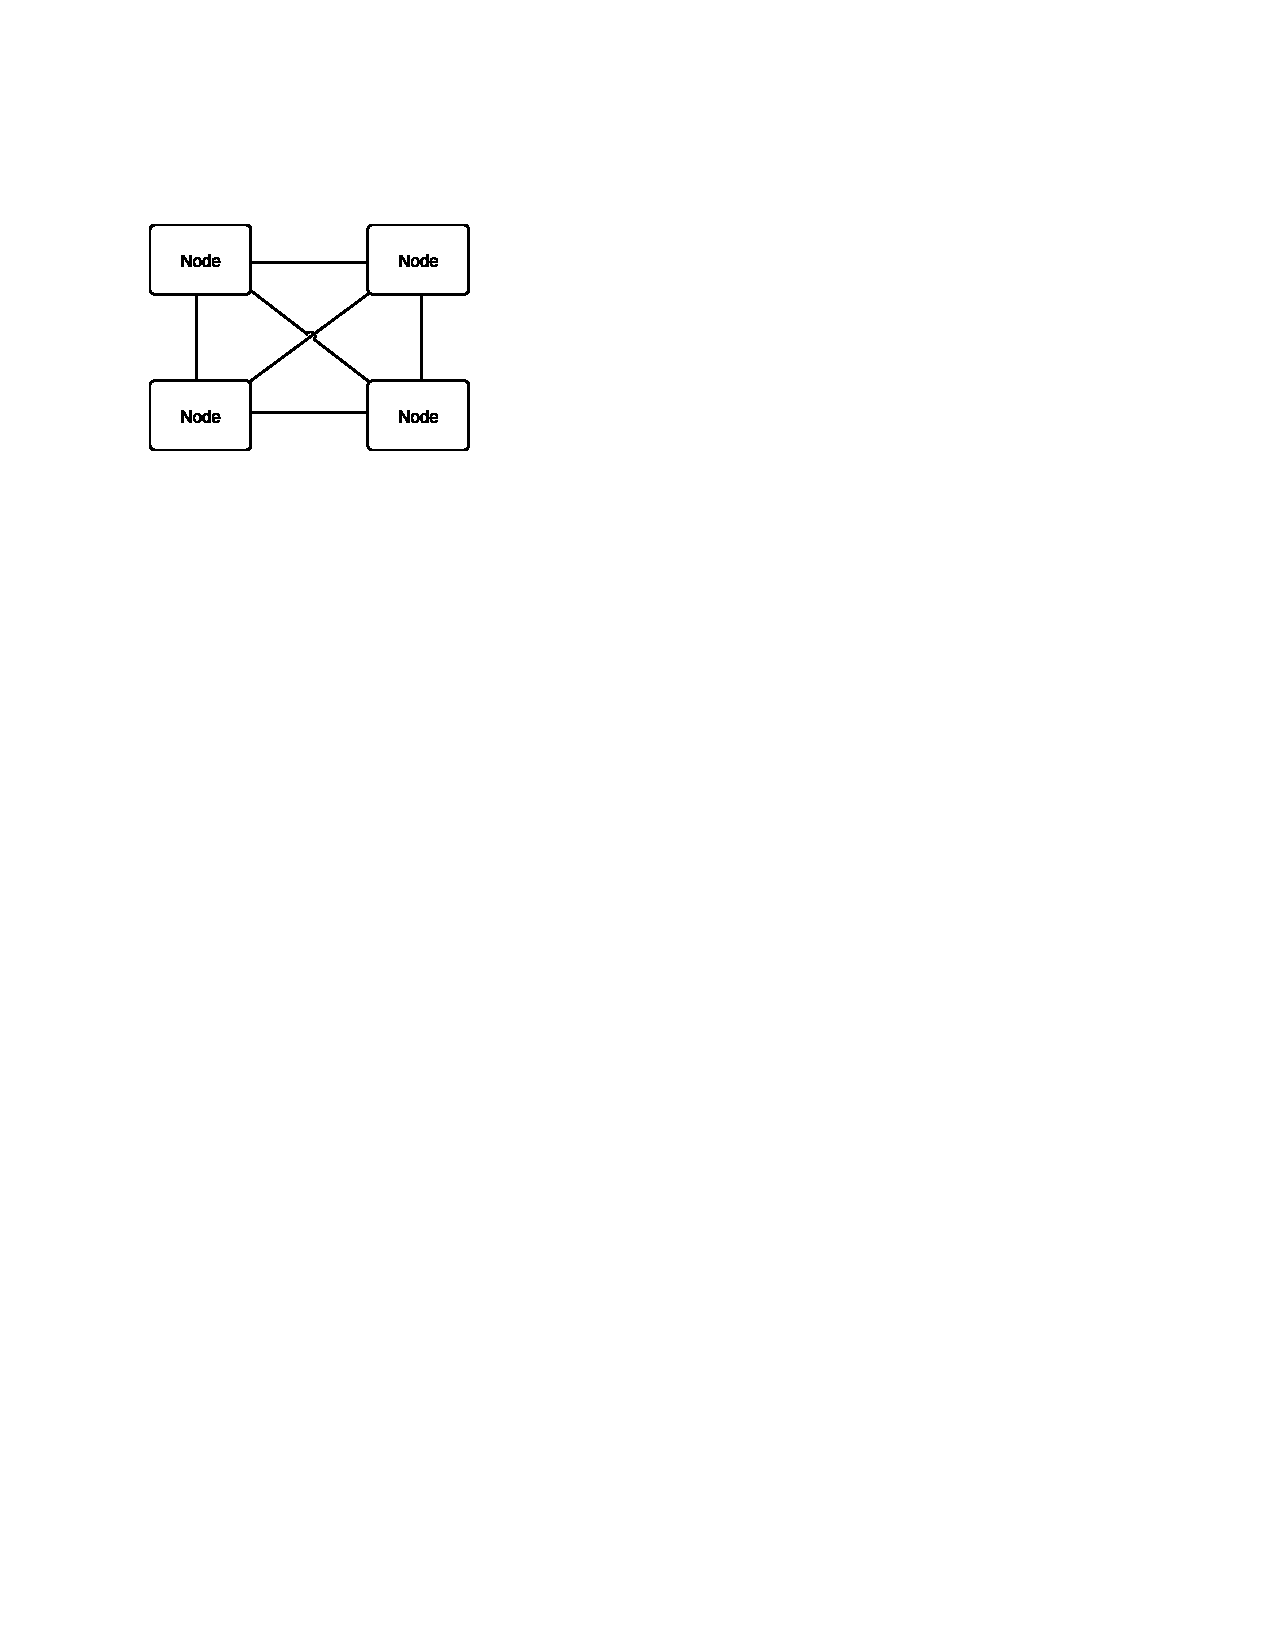
\includegraphics[clip=true, trim= 0 20cm 0 3cm]{fig/Nodes.pdf}
\end{figure}

Erlang hálózatok belső, biztonságos környezetben használatosak, a klaszteren
(\emph{cluster}) kívüli világgal, az interneten keresztül, valamelyik IP alapú
protokollal -- TCP, UDP, SCTP -- lehet kommunikálni. Egy webszolgáltatás
esetében például a belső hálózat Erlang node-okból áll, a külvilág -- a
böngésző -- pedig HTTP protokollon keresztül éri el a HTTP szervert futtató
gépet \citep{ArmstrongThesis}. 

Elosztott rendszereknél bizonyos méret fölött, különösen földrajzilag is
diverzifikált rendszereknél a CAP-elméletnek megfelelően a következő háromból
valamelyiket fel kell adni:
\begin{description}
\item[\emph{Consistency}] \hfill \\
 A rendszer által tárolt adatok mindig, minden pillanatban konzisztensek, a
referenciák érvényesek és minden felhasználó ugyanazt látja. Ha egy darab könyv
van raktáron, és azt valaki megveszi, akkor egy másik vásárló ugyanezt a
könyvet már nem tudja megvenni, azt fogja látni, hogy elfogyott.

\item[\emph{Availability}] \hfill \\
  A kliens mindig kap választ, a rendszer mindig elérhető. A válasz lehet
sikeres vagy sikertelen végrehajtás eredménye is, a lényeg, hogy a kérést
intéző fél mindig kap információt az eredményről.

\item[\emph{Partition Tolerance}] \hfill \\
 Csak a teljes rendszer hibás működése esetén fordulhat elő, hogy a kliens
rossz választ kapjon, vagy egyáltalán ne kapjon választ.
\end{description}

\noindent A fenti korlátozás a rendszer növekedésével párhuzamosan válik
szembetűnővé. Amíg egy gép van (sok-sok redundáns diszkkel), addig minden
konzisztens, viszont a legegyszerűbb hardver hiba is elég, hogy ne legyen
elérhető. Nő a forgalom, a működtető nem akar kiesést, egyre több gépet állít
csatasorba, az adatok nem férnek már el semmilyen számítógépen, elosztott
architektúrára van szükség. Ha az is meg van, akkor felmerül, hogy ha tűz üt ki
az épületben, akkor nem lesz elérhető semmi. Földrajzilag is el kell különíteni
az egyes részeket: ekkor az a probléma, hogy meg kell oldani a konzisztens
adatmódosítást úgy, hogy közben az elérhetőség (elfogadható válaszidő) ne
sérüljön. A CAP-elmélet állítása szerint tehát valamelyik feltétel a háromból
mindenképpen sérül \citep{CAP}.

A dolgozat 4. fejezetben bemutatott alkalmazás esetében az
elérhetőségről (\emph{availability}) mondunk le. A rendszer egy Erlang
node-okból álló klasztert alkot egy biztonságos helyi hálózaton belül,
földrajzilag nincs elkülönítve egyetlen része sem (ez az irány -- nevezetesen a
konzisztencia feladása -- egy későbbi dolgozat tárgya lehet). A rendszer
állapota mindig konzisztens, és a rendszer mindaddig válaszképes, amíg akár
egyetlen node is üzemel.

A dolgozat célja nem egy Google vagy Amazon méretű cég technológiai hátterének
elemzése, hanem az Erlang/OTP platform bemutatása, ezért ezt a feltételt dobjuk
el. Egy így felépíthető rendszer kapacitása, képességei is messze meghaladják
egy átlagos magyar vállalkozás vagy akár egyetemi tanulmányi rendszer
követelményeit. Biztosítani képes a folyamatos működést és az elfogadható
válaszidőt (\emph{soft-realtime}).

\chapter{Az Erlang programozási nyelv alapjai} 
Az ebben a részben bemutatásra kerülő Erlang szintaxis nem fedi le a teljes
nyelvet, a cél, hogy a következőkben bemutatott alkalmazás felépítése, a
modulok érthetőek legyenek.

Minden Erlang folyamathoz tartozik egy \emph{shell}, amely egy REPL (\emph{Read
Eval Process Loop}) alkalmazás a futó környezethez. Ennek segítségével egy
egyszerű parancssoros felületen ki lehet próbálni parancsokat, műveleteket, sőt
-- mint később még látni fogjuk -- ,,éles'' (\emph{production}) környzeteknél
is hozzáférhetünk a rendszerhez (például hibakeresés céljából).

Az Erlang shell indítása után egy \emph{prompt}-ot ad, a sor eleji szám a
beírt kifejezések ('.'-tal bezárólag) sorszámát jelenti. Induláskor:

\begin{code}{}{}
\$ erl -sname a
Erlang R13B03 (erts-5.7.4) [source] [smp:2:2] ...

Eshell V5.7.4  (abort with ^G)
(a@notebook)1> 1 + 2 + 3.
6
(a@notebook)2>
\end{code}

\section{Típusok} Az Erlang dinamikus típusos nyelv (\emph{dynamic typed
programming language}).  A statikus típusos nyelvekkel (pl. Java) szemben a
típusellenőrzés futásidőben (\emph{runtime}) történik, nem fordításkor, nem a
változóknak van típusa, hanem az értékeknek.  Például egy függvény
argumentumánál nem kell deklarálni, hogy milyen típusú paramétert fog kapni,
kaphat bármilyet, az futásidőben derül ki, hogy mit kapott, és azt tudja-e
kezelni. 

Funkcionális nyelv lévén a változó nem igazi változó, csak egyszer kaphat
értéket, utána nem lehet módosítani. Az egyszerűség kedvéért használjuk az
angol \emph{variable} szó magyar megfelelőjét. Az Erlangban a változó nevét
mindig nagy betűvel kell kezdeni.

Egy függvény definíció példa. Egy téglalap területét számolja ki a megadott
oldalaiból.

\begin{code}{erlang}{}
terulet(A, B) -> 
  A * B.
\end{code}

A függvényen belül sem az \texttt{A} sem a \texttt{B} változóhoz nem lehet új
értéket rendelni. Amennyiben ciklusra lenne szükségünk, rekurzióval
kell megoldani.

\subparagraph{Integer} Egész számok: \texttt{100, 3.1415, -5}. Méretét a
memória mérete határozza meg, nincs felső korlát.

\subparagraph{Float} Lebegőpontos számok az IEEE 754 64-bites ábrázolásnak
megfelelően.

\subparagraph{Binary} Byte sorozat.

\subparagraph{Atom} Kis betűvel kezdődő alfanumerikus karaktersorozat. Például:
\texttt{ok, error, true, false}. Nem \emph{string}!

\subparagraph{Fun} Függvény típus. A függvények a többi típushoz hasonlóan
használhatók változók értékeként. \texttt{fun(N) -> N * N  end.}

\subparagraph{Reference} Egyedi azonosító, amely összehasonlítás céljából
állítható elő az Erlang \texttt{make\_ref()} függvényével.

\subparagraph{Pid} Process azonosító.

\subparagraph{Port} Az Erlangon kívüli kommunikáció \texttt{port}-okon
keresztül zajlik. Az Erlang \texttt{open\_port()} függvényével hozható létre
például C-ben megírt könyvtárak használatához.

\subparagraph{List} Lista. Eleme bármilyen változó lehet.
\texttt{[1,2,3,4,5,6]}. Az üres lista jelölése: \texttt{[]}.

\subparagraph{Tuple} Több változó egy egységben való kezelésére szolgál. Az
egyes elemeknek nincs nevük, nem lehet közvetlenül hivatkozni rájuk. Egy
\emph{tuple} bármilyen más változót tartalmazhat, újabb tuple-t is. A
szintaxis: \texttt{\{teglalap, \{2, 3\}\}}. Ez esetben a tuple eleme egy atom
és egy tuple, amely két egész számot tartalmaz.

\subparagraph{Record} A rekord szintaktikai egyszerűsítés tuple-ök
használatához. Egy rekord egy olyan tuple, amelynek az első eleme a rekord
nevét tartalmazó atom. A rekord mezőinek neve van, amelyekkel lehet hivatkozni
az egyes elemekre. Futás közben semmiben sem különböznek a tuple-től, a
programozás megkönnyítésére szolgál. Például:

\begin{code}{erlang}{}
-record(sikidom, { nev, a_oldal, b_oldal}).

terulet(S) ->
  S#sikidom.a_oldal * S#sikidom.b_oldal.
\end{code}

\subparagraph{String} Szintaktikai egyszerűsítés egész számok listájához. A
"kakukk" kifejezés ekvivalens a \texttt{[107,97,107,117,107,107]} és 
\texttt{[\$k,\$a,\$k,\$u,\$k,\$k]} listákkal.

\section{Mintaillesztés (\emph{pattern matching})}
A mintaillesztés nagyon fontos fegyver az Erlang arzenálban. Mintaillesztéssel
lehet egy változónak értéket adni, komplex adatszerkezetből adatot kinyerni,
a vezérlést irányítani. A mintaillesztés általános formája:

\begin{verbatim}
    Pattern = Expression
\end{verbatim}

\noindent A baloldali minta (\emph{pattern}) tartalmazhat bármilyen adattípust,
változót, a jobb oldalon azonban csak olyan változó szerepelhet, amelynek van
értéke. A kifejezés ezen kívül még tartalmazhat műveletet, függvényhívást is. A
mintában szereplő, még értékkel nem rendelkező változó a jobboldali kifejezés
alapján kap értéket. Amennyiben a bal oldalon álló változónak már van értéke, a
mintaillesztés csak akkor lesz sikeres, ha a jobboldali kifejezésben, a
megfelelő helyen, ugyanaz az érték szerepel.

A mintaillesztésnek két eredménye van: vagy sikeres vagy nem. Néhány példa az
egyszerű értékadástól, a komplexebb szerkezetig.

\begin{code}{}{}
1> A = A + 2.
* 1: variable 'A' is unbound
2> A = 2.
2
3> A = A + 2.
** exception error: no match of right hand side value 4
4> B = A + 2.
4
5> B.
4
6> B = A + A.
4
7> B = 2 * A.
4
8> C = A + B.
6
9> C.
6
\end{code}

\noindent Az 1. utasítás nem értelmezhető, mert az \texttt{A} változónak nincs értéke
(\emph{unbound}), és a jobb oldalon nem szerepelhet így (nincs is értelme). A 3.
utasításnál az \texttt{A} változónak van értéke (2), de a mintaillesztés nem
sikeres, mert a bal oldalon így 2 szerepel, a jobb oldalon meg 4.

Listáknál a mintaillesztésnél használható az alábbi szintaxis a lista első
elemének (\emph{head}) kinyerésére.

\begin{verbatim}
    [Head|Tail] = [1,2,3,4,5]
\end{verbatim}

\noindent Ebben az esetben a \texttt{Head} változóban lesz a lista első eleme (1), a
\texttt{Tail} változóban a többi elem listája (\texttt{[2,3,4,5]}). Néhány
példa listás mintaillesztésre:

\begin{code}{}{}
1> List = [1,2,3,4,3,2,1].
[1,2,3,4,3,2,1]
2> [Head|Tail] = List.
[1,2,3,4,3,2,1]
3> Head.
1
4> Tail.
[2,3,4,3,2,1]
5> [H1,H2|T] = List.
[1,2,3,4,3,2,1]
6> H2.
2
7> T.
[3,4,3,2,1]
8> A = 3.
3
9> [1,2,E,4,E,2,1] = List. 
[1,2,3,4,3,2,1]
10> E.
3
11> [1,2,F,4,3,F,1] = List.
** exception error: no match of right hand 
side value [1,2,3,4,3,2,1]
\end{code}

\noindent A 9. utasítás sikeres, mert az \texttt{E} változónak nincs értéke, és
a jobb oldalon lévő lista 3. és 5. eleme megegyezik. A mintaillesztés sikeres,
és az \texttt{E} változó a 3-as értéket kapja. A 11. utasításnál azért nem
sikerül az illesztés, mert az \texttt{F} változó két olyan helyen szerepel a
listában, ahol különböző érték áll a jobboldali kifejezésben.

\noindent Hasonlóképpen a \emph{tuple}-öknél.

\begin{code}{}{}
1> C = {degree, celsius, 37}.
{degree,celsius,37}
2> F = {degree, fahrenheit, 99}.
{degree,fahrenheit,99}
3> 
3> {degree, Type, Value} = C.
{degree,celsius,37}
4> {Type, Value}.
{celsius,37}
\end{code}

\noindent A rekordok valójában tuple-ök, amelyeknek az első eleme a rekord
neve, így a rekordokat is lehet használni a mintaillesztésekben. A fenti példa
rekordra átírva:

\begin{code}{erlang}{}
1> rd(degree, { type, value}).
degree
2> T = #degree{ type=celsius, value=37 }.
#degree{type = celsius,value = 37}
3> #degree{type=celsius} = T.
#degree{type = celsius,value = 37}
4> #degree{type=Type} = T.   
#degree{type = celsius,value = 37}
5> Type.
celsius
6> {degree, celsius, Value} = T.
#degree{type = celsius,value = 37}
7> Value.
37
\end{code}

\noindent A rekord szintaxis több mezőnél válik hasznossá, amikor csak egy-egy
mező értékét szeretnénk kinyerni (és a rekord szintaxisú mintaillesztések akkor
is működni fognak, ha a mezőszám megváltozik, míg tuple-nél az összes helyen
módosítani kellene a kódot, ahol mintaillesztésben szerepel). A 6. utasításnál
látszik, hogy a tuple szintaxisú minta is megfelel a jobboldali rekordnak.

\section{Függvény definiálása} A mintaillesztés a függvények definiálásánál
is nagyon hasznos, a függvény argumentumainak mintát megadva lehet a komplexebb
paraméterből változóknak értéket adni, illetve külön állításokat
(\emph{function clause}) megfogalmazni a függvényhez, milyen input esetén mit
csináljon. Egy névvel és azonos számú argumentummal (\emph{function arity})
egy függvényt lehet definiálni, de azon belül több állítást lehet tenni. Egy
névvel, de eltérő számú argumentummal akármennyi különálló függvényt lehet
definiálni. Az általános szintaxis jól látszik a következő egyszerű példán:

\begin{code}{erlang}{}
convert(celsius, T) ->
  9 * T / 5 + 32;
convert(fahrenheit, T) ->
  5 * (T - 32) / 9;
convert(_,_) ->
  unkown.

convert() ->
  nothing.

convert(A) ->
  A.
\end{code}

A fenti példa három függvény-definíciót tartalmaz. Az egyik a \texttt{convert}
függvény két paraméterrel (Erlangban a jelölése: \texttt{convert/2}), paraméter
nélkül (\texttt{convert/0}) és egy paraméterrel (\texttt{convert/1}). A két
paraméteres függvény három \emph{function clasue}-ból áll: a kapott paraméter
alapján mintaillesztéssel dől el, hogy melyik rész fut le. Az '\texttt{\_}' jel
azt jelenti, hogy ,,bármi'' -- mindenre illeszkedik. Ha tehát a függvényhívás a
következő: \texttt{convert(celsius, 36)}, akkor a legelső számítás eredményét
adja vissza, mert a \texttt{celsius} atom megegyezik a mintával, a \texttt{T}
változó pedig megkapja értéknek a 36-ot.

Anonim függvények definiálása hasonló módon történik, csak ott a név helyett a
\texttt{fun} kulcsszó szerepel, az egyes \emph{function clause}-oknál pedig
csak a zárójelbe írt argumentum lista. Anonim függvényt bárhol definiálhatunk,
ahol változót is írhatnánk.

\begin{code}{erlang}{}
Convert = fun(celsius, T) ->
                  9 * T / 5 + 32;
             (fahrenheit, T) ->
                  5 * (T - 32) / 9;
             (_,_) ->
                  unkown
          end.
\end{code}

Ebben az esetben a \texttt{Convert} változó értéke lesz a függvény, és a következő módon
lehet meghívni: \texttt{Convert(celsius, 36}). Az anonim függvény definiálása
az \texttt{end} kulcsszóval zárul.

Végezetül egy példa egy jellemző rekurzív függvény bemutatására. Az alábbi
\texttt{insert} függvény egy elemet illeszt be egy rendezett listába.

\begin{code}{erlang}{}
insert(I, []) ->
  [I];
insert(I, [H|T]) when I > H ->
  [H | insert(I, T)];
insert(I, [H|T]) ->
  [I, H|T].
\end{code}

\noindent A \texttt{when} kulcsszó utáni feltétel neve: \emph{guard}. Ezzel
lehet tovább finomítani a mintában megfogalmazott feltételeket. Jelen esetben
addig hívja meg újra és újra az insert függvényt (2. \emph{function clause}),
amíg a beillesztendő elem nagyobb az aktuális listaelemnél (folyamatosan a
lista elejére téve a megvizsgált listaelemet). Amikor ez a feltétel nem
teljesül, akkor beilleszti a fennmaradó lista elejére az elemet, és nem
vizsgálódik tovább (3.  \emph{function clause}). Az egyes lépések eredményei
egy rövid kis listán:

\begin{code}{}{}
1> list:insert(4, [1, 3, 4, 6]).
3. function clause [4,4,6]
2. function clause [3,4,4,6]
2. function clause [1,3,4,4,6]
[1,3,4,4,6]
2> list:insert(7, [1, 3, 4, 6]).
1. function clause [7]
2. function clause [6,7]
2. function clause [4,6,7]
2. function clause [3,4,6,7]
2. function clause [1,3,4,6,7]
[1,3,4,6,7]
\end{code}

\noindent A \texttt{list:insert} kifejezés jelentése: a \texttt{list} modulban
lévő \texttt{insert} függvény. 

\section{Modulok} A modulok szolgálnak logikailag összetartozó függvények
csoportosítására. A modulok nem alkotnak hierarchiát (\emph{flat namespace}),
elnevezéssel lehet megoldani a szükséges tagolást. A modulokban az alábbi
részek szerepelhetnek:

\begin{itemize}
\item modul attribútumok, verziószám, szerző, név, interfész függvények
deklarálása;
\item rekord, makró definíciók, külső fájlok (\emph{header}) beillesztése;
\item függvények.
\end{itemize}

\noindent Egy egyszerű modul:

\begin{code}{erlang}{}
-module(temp).
-export([convert/1]).

convert({celsius, T}) when is_number(T) ->
  {fahrenheit, c2f(T)};
convert({fahrenheit, T}) when is_number(T) ->
  {celsius, f2c(T)};
convert(_) ->
  bad_parameter.

f2c(F) ->
  5 * (F - 32) / 9.
c2f(C) ->
  9 * C / 5 + 32.
\end{code}

A fenti modul az egy argumentummal rendelkező \texttt{convert} függvényt
exportálja, csak ezt lehet meghívni más modulokból. A modul neve \texttt{temp},
kötelező ugyanilyen nevű fájlba tenni.

\section{Konkurens programozás}
Az Erlangban a fentebb röviden bemutatott aktor modellen alapul a párhuzamos
programozás. Az aktorok \emph{process}-ek, amelyek tudnak üzenetet
fogadni (\emph{receive}) és küldeni (\emph{send}). A process az Erlang VM
fennhatósága alá tartozik, nem külön operációs rendszer folyamat, indítása nem
igényel sok erőforrást, egy-egy rendszeren belül akár több százezer process-t
is lehet indítani. Például egy HTTP szerver megvalósítása lehet az, hogy minden
kapcsolathoz tartozik egy önálló webszerver process. Ha ebben valami hiba
történik (pl. 0-val osztás), akkor ez a process leáll, a többi működik tovább
\citep{CesariniBook}.

Process-ek programozásához az eddigieken bemutatottakon túl mindössze három
műveletre van szükség:

\subparagraph{Process indítása} Process-t a \texttt{spawn} függvénnyel lehet
indítani helyben vagy akár egy másik node-on.
\begin{code}{erlang}{}
 P = spawn(module, function, [P1, P2 ...]).
\end{code}

\noindent A process-ek egyedi azonosítót kapnak, amely a címük, ide lehet
küldeni az üzenetet. Van lehetőség arra is, hogy a process nevet kapjon, ezt
hosszabb ideig futó processeknél érdemes megtenni.

\subparagraph{Üzenet küldése} Üzenetet küldeni a következők szerint lehet:
\begin{code}{erlang}{}
          P ! "Hello". 
\end{code} 
\noindent ahol \texttt{P} a process azonosítója vagy regisztrált
neve, a \texttt{!} a küldés operátor. A jobb oldalon álló kifejezés az üzenet,
amely nem csak \emph{string} lehet, mint a fenti példában, hanem bármilyen Erlang
kifejezés (tuple, fun, lista, stb). Másik node-ra ugyanígy lehet üzenetet
küldeni, nincs különbség.

\subparagraph{Üzenet fogadása} A \texttt{receive} utasítás szolgál az üzenetek
fogadására. 
\begin{code}{erlang}{}
receive
  Pattern1 ->
        ...;
  Pattern2 ->
        ...;
  _ ->
        ...;
after Time ->
        ...
end.
\end{code}

\noindent A függvényekhez hasonlóan \emph{clause}-okat tartalmaz, és itt is
mintaillesztés alapján dől el, melyik ág fog lefutni. Minden process-hez
tartozik egy \emph{mailbox}, amelyből a \texttt{receive} utasítással lehet kiolvasni az
üzeneteket. Az utasítás addig olvassa a mailbox-ot, amíg nem talál egy olyan
üzenetet, amely illeszkedik valamelyik ág mintájára. Ekkor kiolvassa, és az
üzenet törlődik a mailbox-ból. Ha egyik mintára sem illeszkednek a beérkező
üzenetek, akkor előbb-utóbb megtelik a memória. Éppen ezért szokás a legtöbb
esetben az utolsó ág mintáját '\_'-ként megadni. Ez a minta mindenre
illeszkedik, így végül minden üzenet törlődik a mailbox-ból. Az \texttt{after}
utasítással meg lehet adni, hogy ha \texttt{Time} ideig nem érkezett olyan
üzenet, ami valamelyik mintára illeszkedett, akkor mit hajtson végre a program
(\emph{timeout}).

Az egyes process-ek -- azonkívül, hogy tudnak egymásnak üzeneteket küldeni --
monitorozni is tudják egymást, nem múlt-e ki a másik. Ennek módja a process-ek
összekapcsolása a \texttt{link} függvénnyel. 

\begin{code}{erlang}{}
start() ->
  process_flag(trap_exit, true),
  Pid = spawn(module, function, []),
  link(Pid),
  receive
    {'EXIT', Pid, Reason} ->
      io:format("Process ~p has just died.~n", [Pid])
  end.
\end{code}

A fenti \texttt{start} függvény elindít egy másik process-t és összekapcsolja a
jelenlegivel. Amikor a másik process leáll, érkezik egy üzenetet erről, aminek a
formátumát a fenti \texttt{receive} blokkban szereplő mintán lehet látni. 

Ahhoz, hogy egy process folyamatosan fusson, újra és újra meg kell hívni a
\texttt{receive} utasítást (hogy várakozzon üzenetre). Az alábbi modul egy
process-t futtat, amíg egy \texttt{stop} atomot nem kap üzenetként. A
\texttt{?MODULE} makró a modul nevét tartalmazza.

\begin{code}{erlang}{}
-module(temp).
-export([start/0, loop/0]).

start() ->
  spawn(?MODULE, loop, []).

loop() ->
  receive
    {From, celsius, T} ->
        From ! {fahrenheit, c2f(T)},
        loop();
    {From, fahrenheit, T} ->
        From ! {celsius, f2c(T)},
        loop();
    stop ->
      stopped;
    _ ->
      loop()
  end.

f2c(F) ->
  5 * (F - 32) / 9.

c2f(C) ->
  9 * C / 5 + 32.
\end{code}

A puding próbálja az evést -- az Erlang shellben. A \texttt{self()} függvény az
aktuális process azonosítóját adja vissza, jelen esetben az shell-ét; a
\texttt{flush()} shell-utasítás pedig kilistázza és törli a shell mailbox-át.

\begin{code}{}{}
1> c(temp).
{ok,temp}
2> P = temp:start().
<0.42.0>
3> P ! {self(), fahrenheit, 99.9}.
{<0.35.0>,fahrenheit,99.9}
4> flush().
Shell got {celsius,37.72222222222222}
ok
5> P ! stop.                      
stop
6> flush(). 
ok
7> P ! {self(), fahrenheit, 99.9}.
{<0.35.0>,fahrenheit,99.9}
8> flush().                       
ok
\end{code}

Az ebben a részben bemutatott téglákból építkezik az Erlang részét képező,
a leggyakoribb feladattípusok megoldására létrehozott Open Telecom Platform 
(OTP) szoftverkönyvtár, amely központjában a magas rendelkezésre állású,
párhuzamos rendszerek építése áll.

\section{Open Telecom Platform (OTP)} Nagyobb szoftverek fejlesztésekor
elkerülhetetlen, hogy a fejlesztők valamilyen közös implementációs gyakorlatot
kövessenek. Enélkül minden egyes fejlesztő kitalálja magának a világ legjobb
megoldását (és ebben rendkívül kreatívak tudnak lenni), amit rajtuk kívül senki
más nem ért. Az OTP formalizált keretet ad a process-fejlesztéshez. Hasonlóan a
Java EE \emph{servlet}-eihez, egy interfészt definiál, amelyet minden Erlang
fejlesztő ért, így a rendszer különböző emberek által fejlesztett részei egy
koherens egészet alkotnak. Ezek mögött az interfészek mögött ráadásul általános
problémák megoldásai állnak, nem kell újra és újra kitalálni például a
hibakezelés módját.

Az OTP viselkedésmintákat definiál (\emph{behaviour}), amelyekhez a megadott
\emph{callback} függvényeket (a Java interfész függvényeinek implementálásához
lehet hasonlítani) implementálva egy process-modul hozható létre. Ezt a modult
az OTP kezeli, és adott eseménynél meghívja a megfelelő függvényt. Az OTP-ben a
process-ek hierarchiába rendezhetők, ennek megfelelően van háromféle típusú
process.

\subparagraph{Application} Az OTP application \emph{behaviour} egy Erlang/OTP
alkalmazás, amely összefogja a modulok egy csoportját, és a process-hierarchia
csúcsán áll.

\subparagraph{Supervisor} Olyan \emph{behaviour}, amelynek feladata más processek
felügyelete, folyamatosan monitorozza azok állapotát, észleli, ha
a processben hiba történt, és a megadott újraindítási stratégiának megfelelően
újraindítja vagy hagyja leállni. Supervisor processek alá tartozhatnak
\emph{worker} és további supervisor processek.

\subparagraph{Worker} Olyan process, amely valamilyen alkalmazás-specifikus
feladatot végez, nem felügyel más process-eket. Az OTP az alábbi
\emph{behaviour}-öket biztosítja:
\begin{itemize}
\item \emph{Generic server (gen\_server)}: általános szerver;
\item \emph{Generic Finit State Machine (gen\_fsm)}: véges automata;
\item \emph{Generic Event Handler (gen\_event)}: események, alarmok kezeléséhez;
\end{itemize}

\citep{OTPInAction}.

\newpage
A fenti celsius-fahrenheit átváltó modul \emph{gen\_server} átirata:

\begin{code}{erlang}{}
-module(temp_otp).
-behaviour(gen_server).

-export([start/0]).
-export([init/1, handle_call/3, handle_cast/2, 
         handle_info/2, code_change/3, terminate/2]).

start() ->
  gen_server:start_link({local, ?MODULE}, ?MODULE, [], []).

init(_Options) ->
  {ok, 0 }.

handle_cast({From, celsius, T}, State) ->
  From ! {fahrenheit, c2f(T)},
  {noreply, State + 1};
handle_cast({From, fahrenheit, T}, State) ->
  From ! {celsius, f2c(T)},
  {noreply, State + 1};
handle_cast(stop, State) ->
  io:format("Server handled ~p requests.~n", [State]),
  {stop, normal, State};
handle_cast(_Info, State) ->
  {noreply, State}.

handle_call({celsius, T}, _From, State) ->
  {reply, {fahrenheit, c2f(T)}, State + 1};
handle_call({fahrenheit, T}, _From, State) ->
  {reply, {celsius, f2c(T)}, State + 1}.

handle_info(_Info, State) ->
  {noreply, State}.

terminate(_Reason, _State) ->
  ok.

code_change(_OldVsn, State, _Extra) ->
  {ok, State}.

f2c(F) ->
  5 * (F - 32) / 9.
c2f(C) ->
  9 * C / 5 + 32.
\end{code}

A fenti modul egy szerver, amely kétféleképpen használható: szinkron
(\texttt{handle\_ call} callback függvény) és aszinkron (\texttt{handle\_cast})
módon. Indításkor a modul nevén regisztráljuk a process-t
(\texttt{gen\_server:start\_link}), így process azonosító helyett erre a névre
is lehet címezni az üzeneteket. A szervernek háromféleképpen lehet üzenetet
küldeni: a \texttt{gen\_server:cast()} és \texttt{gen\_server:call()}
függényekkel, és a standard módon a \texttt{!} operátorral (ezt az esetet a
\texttt{handle\_info()} függvénnyel lehet kezelni).

A függvények megkapják az \texttt{init} függvényben inicializált \texttt{State}
paramétert (jelen esetben egy egész számot) minden egyes hívásnál. Ez a változó
használható a szerver állapotának tárolására, a példában az elvégzett
konverziók számát tartalmazza, amit leállításkor kiír. Próba a shell-ben:

\begin{code}{}{}
1> c(temp_otp).
{ok,temp_otp}
2> temp_otp:start().
{ok,<0.42.0>}
3> gen_server:cast(temp_otp, {self(), celsius, 37}).
ok
4> flush().
Shell got {fahrenheit,98.6}
ok
5> {fahrenheit,F}=gen_server:call(temp_otp, {celsius, 37}).
{fahrenheit,98.6}
6> F.
98.6
7> gen_server:cast(temp_otp, stop).                           
Server handled 2 requests.
ok
\end{code}

A fenti példában a szerver nem része semmilyen process hierarchiának, nem
felügyeli \emph{supervisor} a működését. A kód bonyolultabbnak tűnhet a nem OTP-s
megoldásnál, de ahogy nem egy ennyire egyszerű, teljesen egyedülálló szerver
process-ről van szó, az OTP-s környezet hamar behozza az árát. Erre nézünk egy
kicsit összetettebb, de azért még követhető példát a következő fejezetekben.

\chapter{Tőzsdei ,,ticker'' alkalmazás} Állatorvosi lóként egy egyszerű
üzenetküldésen alapuló webes szolgáltatást fogunk megvizsgálni, ezen mutatjuk
be az eddigiekben leírtak alkalmazását egy kicsi ám működőképes rendszer
megalkotásában. A rendszer célja, hogy a tőzsde felöl érkező pillanatnyi
kereskedési adatokat (melyik részvényből milyen áron hány darabot adtak el az
adott tranzakció során) a weben keresztül eljuttasa a felhasználóknak. A webes
felület lehet akár egy előfizetői oldal, ahol a tőzsdei adatok real-time
jelennek meg, vagy lehet egy újság, ahol a szokásos 15 perces késleltetéssel
lehet látni az árakat. A rendszerrel szemben támasztott elvárások:
\emph{soft-realtime} működés, magas rendelkezésre állás, belátható üzemeltetési
költségek. A dolgozat terjedelmi korlátai és az átláthatóság miatt nem térünk
ki minden egyes részletre, nem faragunk csicsás weboldalt, de a fenti
elvárásokat kielégítő megoldásokat mind bemutatjuk.

A magas rendelkezésre állás követelményéből fakadóan egynél több gépre lesz
szükség. Az egyszerűség és a terminológia kedvéért az alábbiakban Erlang
node-ként hivatkozunk az egyes gépekre.

A tőzsdei kereskedési rendszer kívül esik a látókörünkön, az adatokat
egyszerűen inputként kezeljük, melyek Erlang üzenet formájában érkeznek. A
tőzsdei kereskedést egy egyszerű véletlenszám-generátorral dolgozó process
szimulálja.

A feladat magját jelentő üzenetküldés-kezelő rendszert egy külön, általánosan
használható szerverként implementáljuk, erre építjük a webes felületet nyújtó
egyszerű kis webalkalmazást.

\section{ZM -- üzenetküldés, fogadás}
A ZM fantázinevű alkalmazás egy \emph{publish-subscribe} rendszer, amely
csatornákat (\emph{channel}) definiál, amelyekre fel lehet iratkozni
(\emph{subscribe}), és amelyekre üzenetet lehet küldeni (\emph{publish}). A ZM
szerver biztosítja, hogy az egyes csatornákhoz küldött üzenetet megkapják az
előfizetők (,,akik'' maguk is process-ek) függetlenül attól, hogy melyik gépen
küldték az üzenetet, és kezeli a csatornák működésében előforduló hibákat. A ZM
keretet ad alkalmazásoknak, amelybe be lehet illeszteni az adott alkalmazás
saját csatorna-implementációit (\emph{gen\_server}-ként). Így az üzenetküldés
szolgáltatás egyszerűen beilleszthető például egy webes szolgáltatásba,
használatához csak a csatornákat kell implementálni.

\section{Felépítés}
A ZM szerver felépítése az OTP alapelveknek felel meg, az egyes feladatokat
önálló processek végzik, a processek hierarchiát alkotnak, ahol
supervisor-ok felügyelik az alattuk futó folyamatokat. Az alábbi ábrán néven
nevezzük az egyes elemeket.

\begin{figure}
\caption{A ZM alkalmazás process-hierarchiája}
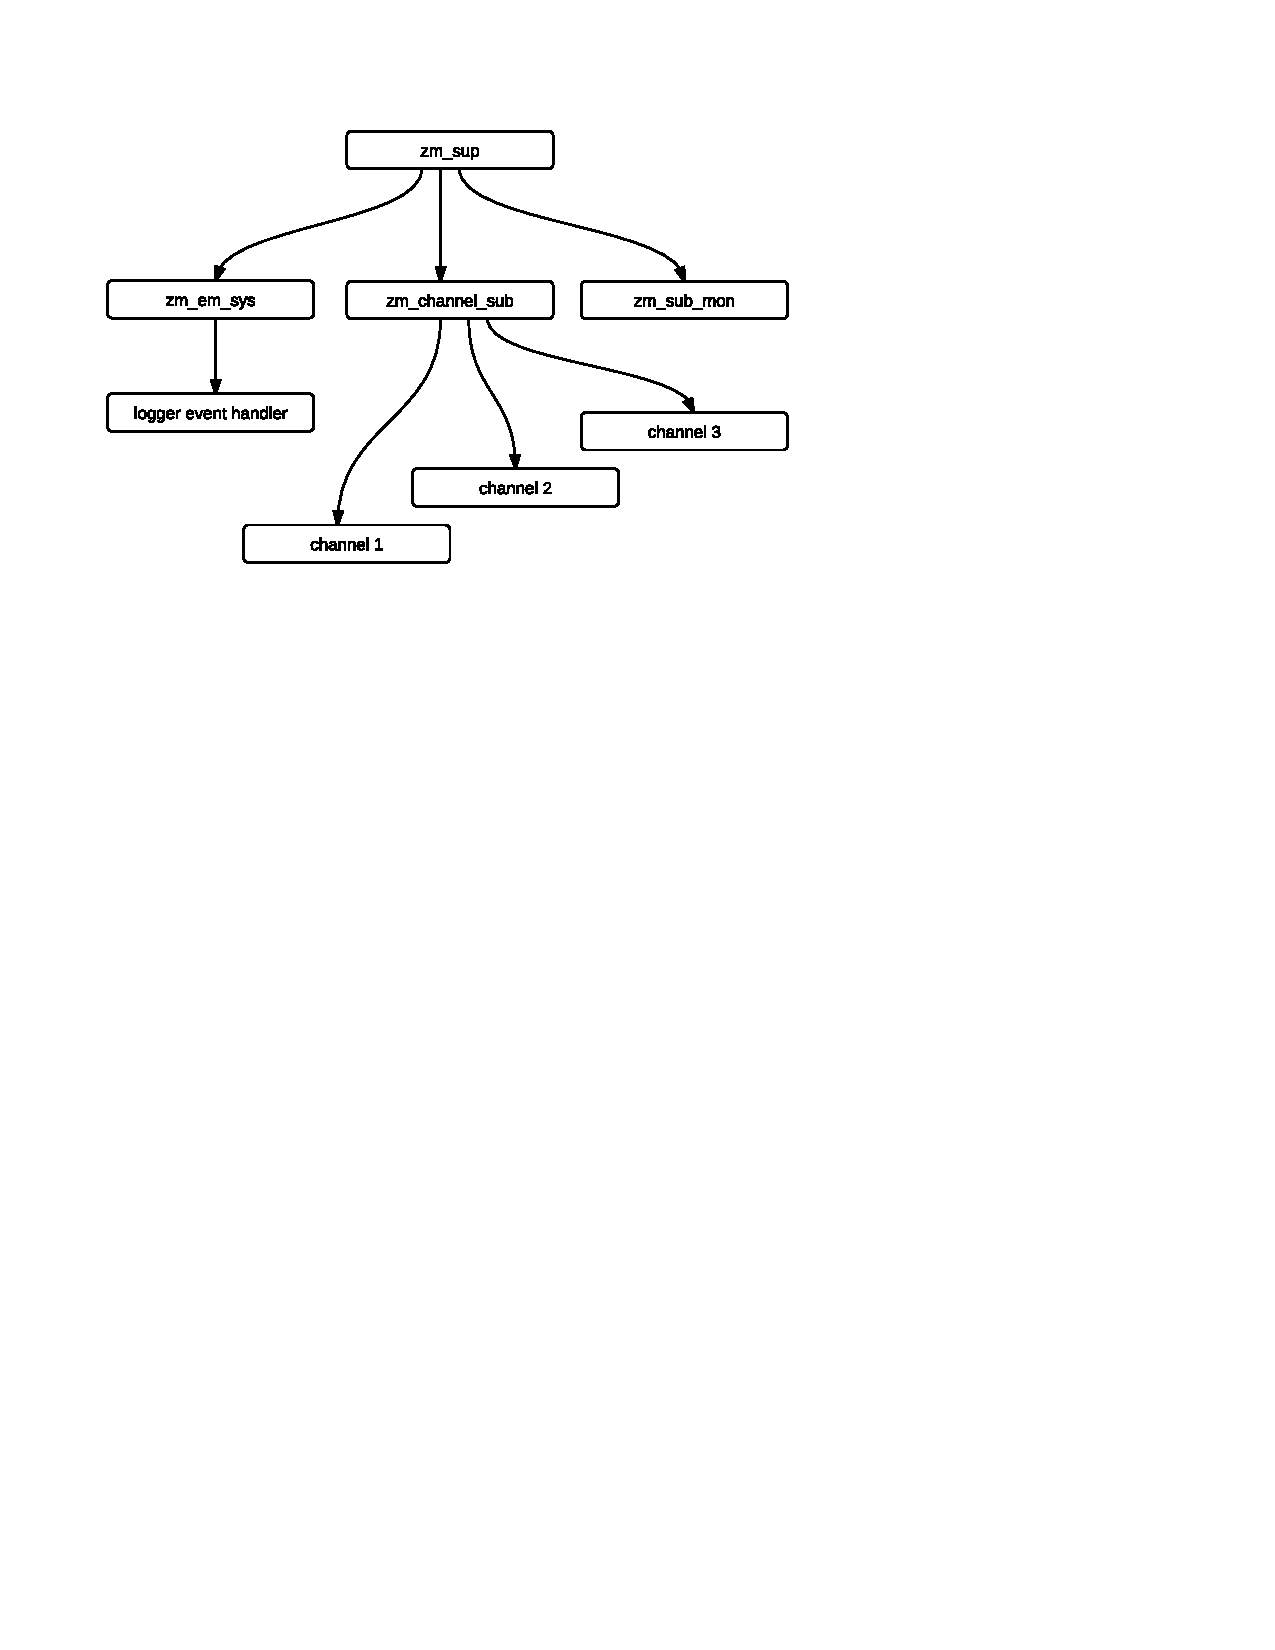
\includegraphics[clip=true, trim= 0 18cm 0 1cm]{fig/ZmSup.pdf}
\end{figure}

\subparagraph{zm\_sup} A gyökere a process-fának. Ez a supervisor kezeli az
alábbi három folyamatot. Újraindítási stratégiája: \emph{one\_for\_one}, ami
azt jelenti, hogy ha valamelyik process leáll, akkor azt az egyet indítja újra,
a többivel nem foglalkozik.

\subparagraph{zm\_em\_sys} \emph{Event manager}, amely eseményeket fogad,
és azokat a hozzácsatolt \emph{event handler}-eknek továbbítja. A rendszer
működése során a számottevő eseményekről értesíti (\emph{notify}) ezt a
process-t, és például egy hozzácsatolt naplózó (\emph{logger}) handler egy
fájlban rögzíti a tényt. A ZM nem tartalmaz \emph{handler}-t, azt az
alkalmazásra bízza.

\subparagraph{zm\_channel\_sup} Supervisor, amely a csatorna process-eket
felügyeli. Minden elindított csatorna ez alá a folyamat alá kerül, a
\texttt{zm\_channel\_sup} indítja, állítja le, monitorozza őket.

\subparagraph{zm\_sub\_mon} A feliratkozásokat kezeli, és monitorozza. Ha egy
előfizető folyamat (\emph{subscriber}) véget ér (rendben vagy rendellenesen),
akkor ez a process gondoskodik arról, hogy a csatornák ne küldjenek erre a
címre több üzenetet.

A fenti négy process alkotja a rendszert, ehhez lehet különböző csatornákat
írni. A ZM szerverhez tartozik két egyszerű csatorna-implementáció. Az egyik
egyszerűen csak továbbítja az előfizetők felé az üzeneteket, az előfizető a
felirakozáskor megadhat egy szűrő függvényt (\emph{filter function}), amelyet
minden üzenetre lefuttat a csatorna, és csak akkor továbbítja, ha a függvény
visszatérési értéke \texttt{true}. A másik egy késleltetett csatorna
(\emph{delayed}), amely a beérkező üzenetet a feliratkozáskor megadott
időtartam után küldi csak tovább. Ezzel lehet például biztosítani a tőzsdei
adatoknál szükséges 15 perces késleltetést (előfizetéstől függően ez lehet
real-time adatközlés is).

A csatornák megvalósítása egy-egy \emph{gen\_server} modul. A behaviour-höz
tartozó \emph{callback} függvények implementálása után az alábbi paranccsal indítható.

\begin{code}{}{}
zm_channel:start(zm_ch_delayed, stock_exchange, []).
\end{code}

Ebben az esetben a \texttt{zm\_ch\_delayed} modulban implementált csatorna indul el
\texttt{stock\_ exchange} néven. A \texttt{zm\_ch\_delayed} modul \texttt{handle\_cast}
függvénye (aszinkron a csatornáknak való üzenetküldés). 

\begin{code}{erlang}{}
handle_cast({msg, {_Timestamp, _} = Message}, 
            #state{ id=ChannelId } = State) ->
  Send = fun
    ({SubPid, SubscriptionRef, []}, _) ->
      SubPid ! {msg, {ChannelId, SubscriptionRef}, Message},
      sent;
    ({SubPid, SubscriptionRef, [{delay, Delay}]}, _) ->
      erlang:send_after(timer:minutes(Delay), 
                        SubPid, 
                        {msg, {ChannelId, SubscriptionRef}, 
                        Message}),
      delayed;
    ({_SubPid, _SubscriptionRef, _}, _) ->
      invalid_option
  end,
  zm_sub_mon:fold_subs(ChannelId, {0, 0, 0}, Send),
  {noreply, State};

handle_cast(_Info, State) ->
  {noreply, State}.
\end{code}

Leszámítva a \texttt{gen\_server} alapértelmezett callback függvényeit, a fenti
\texttt{handle\_cast} jelenti a tőzsdei adatok szétküldésére szolgáló
csatornát. A \texttt{Send} változóhoz rendelt függvényt a
\texttt{zm\_sub\_mon:fold\_subs()} hívás minden egyes előfizetőre végrehajtja. A
feliratkozásnál egy opciót lehet megadni: azt, hogy hány perces késleltetéssel
kapja meg az előfizető az adatokat. Egy példa a shell-ben többet mond ezer
szónál: 

\begin{code}{}{}
(zm@notebook)1> zm_channel:start(zm_ch_delayed, 
                                 stock_exchange, []).
{[{ok,started}],[]}
(zm@notebook)2> zm_channel:subscribe(stock_exchange, 
                                     self(), []).   
#Ref<0.0.0.443>
(zm@notebook)3> zm_channel:send(stock_exchange, 
                      {msg, {erlang:now(), "SHARE_1 15"}}),
(zm@notebook)3> receive
(zm@notebook)3> M -> M
(zm@notebook)3> end.
{msg,{stock_exchange,#Ref<0.0.0.443>},
     {{1335,128575,402055},"SHARE_1 15"}}
\end{code}

A fenti \emph{subscribe} eredménye egy real-time előfizetés, a beérkező
üzenetet azonnal kiküldi a csatorna. A késleltetett előfizetéshez a
\texttt{subscribe} függvényben meg kell adni a késleltetés időtartamát.

\begin{code}{}{}
zm_channel:subscribe(stock_exchange, self(), [{delay, 15}]).
\end{code}

Így az üzeneteket 15 perccel érkezés után továbbítja a \texttt{stock\_exchange}
csatorna. De mi történik, ha hiba van? Hol a hibakezelés a fenti
\texttt{handle\_cast} függvényből?

\section{Hibatűrés}
Az Erlang fejlesztési gyakorlatra nem jellemző a defenzív (hibavizsgálattól
függő elágazások a kódban) programozás. Az ajánlott módszer az, hogy a
függvényekben feltételezzük, hogy az input adatok helyesek, és nem írjuk körül
a lehetőségeket, ha valami mégsem lenne megfelelő. Egyetlen kivétel a
felhasználó által megadott adatok bekérésére szolgáló függvények, ott
elkerülhetetlen a vizsgálódás, hiszen ki kell tudni írni, mi a baj a megadott
adatokkal \citep{ArmstrongThesis}.

A hibákat a kódban nem kell kezelni, egyszerűen hagyni kell a process-t
elbukni, és a supervisor-ra bízni a döntést, újraindítja-e a process-t vagy
sem. A hiba úgy derül ki függvényhívásnál, hogy a várható értéket adjuk meg
baloldali mintaként. Amennyiben a függvény nem a várt értéket adja vissza, a
minta nem illeszkedik, és az hiba -- a process leáll (\emph{crash}). A
supervisor ezt észreveszi, meghívja a gen\_server \texttt{terminate}
függvényét, majd újraindítja a process-t. Ha adott időn belül túl sokszor
fordulna elő hiba, akkor nem próbálkozik újra.

A hibakezelést az alábbi függvénnyel teszteljük. A csatornának üzenetként
küldött \texttt{crash} atom nullával való osztást eredményez, amitől leáll a
folyamat.

\begin{code}{erlang}{}
...
handle_info(crash, State) ->
  1 / 0, 
  {noreply, State};
...
terminate(Reason, _S) ->
  io:format("Channel terminated. Reason: ~p~n", [Reason]),
  terminate.
\end{code}

A supervisor azonnal újraindítja a csatornát, és meghívja a modul
\texttt{terminate} függvényét (ahol most csak egy konzol kiírás van, hogy
látható legyen, valóban ez történik). Lássuk a shell-ben.

A csatorna indítása:
\begin{code}{}{}
(zm@notebook)1> zm_channel:start(zm_ch_delayed, 
                                 stock_exchange, []).
...
{[{ok,started}],[]}
(zm@notebook)2> zm_channel:list().
[stock_exchange]
\end{code}

A shell process feliratkozása a csatornára, majd egy üzenet küldés-fogadás --
működik a csatorna:

\begin{code}{}{}
(zm@notebook)3> zm_channel:subscribe(stock_exchange, 
                                     self(), []).   
#Ref<0.0.0.498>
(zm@notebook)4> zm_channel:send(stock_exchange, 
                   {msg, {erlang:now(), "Kakukk"}}).
abcast
(zm@notebook)5> flush().                                                         
Shell got {msg,{stock_exchange,#Ref<0.0.0.498>},
               {{1335,179193,696571},"Kakukk"}}
ok
\end{code}

\emph{Crash} előidézése. Az üzenetküldés után azonnal jön a jelentés, hogy a
\texttt{stock\_ exchange} csatornában hiba történt (jelen esetben:
\texttt{badarith} -- aritmetikai). A \texttt{Channel terminated}
kezdetű kiírást a fentebb bemutatott \texttt{terminate} függvénynek
köszönhetjük.

\begin{code}{}{}
(zm@notebook)6> stock_exchange ! crash.                                          
crash
Channel terminated. Reason: {badarith,
    [{zm_ch_delayed,handle_info,2},
    {gen_server,handle_msg,5},
    {proc_lib,init_p_do_apply,3}]}
(zm@notebook)7> 
=ERROR REPORT==== 23-Apr-2012::13:07:02 ===
** Generic server stock_exchange terminating 
** Last message in was crash
** When Server state == {state,stock_exchange}
** Reason for termination == 
** {badarith,[{zm_ch_delayed,handle_info,2},
              {gen_server,handle_msg,5},
              {proc_lib,init_p_do_apply,3}]}

=CRASH REPORT==== 23-Apr-2012::13:07:02 ===
 crasher:
  initial call: zm_ch_delayed:init/1
  pid: <0.121.0>
  registered_name: stock_exchange
  exception exit:{badarith,[{zm_ch_delayed,handle_info,2},
                            {gen_server,handle_msg,5},
                            {proc_lib,init_p_do_apply,3}]}
  in function  gen_server:terminate/6
  ancestors: [zm_channel_sup,<0.102.0>,<0.86.0>]
  messages: []
  links: [<0.104.0>]
  dictionary: []
  trap_exit: false
  status: running
  heap_size: 377
  stack_size: 24
  reductions: 584
 neighbours:
\end{code}

A supervisor is küldi a jelentést arról, hogy észlelte a hibát, és arról is,
hogy újraindította a csatornát:

\begin{code}{}{}
=SUPERVISOR REPORT==== 23-Apr-2012::13:07:02 ===
     Supervisor: {local,zm_channel_sup}
     Context:    child_terminated
     Reason:     {badarith,[{zm_ch_delayed,handle_info,2},
                            {gen_server,handle_msg,5},
                            {proc_lib,init_p_do_apply,3}]}
     Offender:   [{pid,<0.121.0>},
                  {name,stock_exchange},
                  {mfa,{zm_ch_delayed,start_link,
                        [stock_exchange,[]]}},
                  {restart_type,transient},
                  {shutdown,5000},
                  {child_type,worker}]


=PROGRESS REPORT==== 23-Apr-2012::13:07:02 ===
          supervisor: {local,zm_channel_sup}
             started: [{pid,<0.136.0>},
                       {name,stock_exchange},
                       {mfa,{zm_ch_delayed,start_link,
                            [stock_exchange,[]]}},
                       {restart_type,transient},
                       {shutdown,5000},
                       {child_type,worker}]
\end{code}

Ezután megint működik minden, mint a hiba előtt:

\begin{code}{}{}
(zm@notebook)8> zm_channel:list().                                               
[stock_exchange]
(zm@notebook)9> zm_channel:send(stock_exchange, 
                    {msg, {erlang:now(), "Kakukk again"}}).
abcast
(zm@notebook)10> flush().                                                               
Shell got {msg,{stock_exchange,#Ref<0.0.0.498>},
               {{1335,179242,712806},"Kakukk again"}}
ok
\end{code}

Ez a mechanizmus teszi lehetővé, hogy a modulokban ne kelljen a
hibakezelést mindenhol leprogramozni. Ennek eredményeképpen a kód átláthatóbb
marad, és kevesebb sorból is áll. Kevesebb kód, kevesebb hibalehetőség. 

\section{Hibakeresés}
Hiba, nem dokumentált kódrész azonban mindig marad. Többféle lehetőség közül
választhat a fejlesztő, amikor hibát keres: 
\subparagraph{Debug} A kód futtatása közben vizsgálhatja a fejlesztő a
program-változókat. Hátránya, hogy ,,éles'' környezetben nem igazán
alkalmazható, egy webszolgáltatást nem lehet fejlesztői környezetből futtatni.
\subparagraph{Logging} Minden rendszer elengedhetetlen része a különböző
részletezettségű naplózás. A naplófájlokban rögzíti a rendszer azokat az
eseményeket, amelyek vagy audit vagy hibakeresések miatt érdekesek. Fentebb már
volt szó a ZM program \texttt{zm\_em\_sys} \emph{event\_manager}-eréről, amely
rendszer-eseményeket fogad. Az alkalmazásíró hozzáadhat akármennyi
\emph{event\_handler}-t, amelyekkel például naplózhatja az eseményeket.
\subparagraph{Trace} Az Erlang lehetőséget ad arra, hogy egy aktív node
működését, egészen pontosan függvényhívásait kívülről meg lehessen vizsgálni.
Meg lehet adni, hogy melyik modul melyik függvényére vagyunk kíváncsiak, és meg
lehet adni a paraméterek mintáját is, hogy csak azokat a hívásokat kapjuk meg,
amik érdekelnek -- elkerülendő a több gigabájtos, áttekinthetetlen eredményt. 

A trace nagy előnye, hogy ,,éles'' környezetben is használható, a szoftver
megfigyelhető futás közben. Ez különösen akkor hasznos, amikor nem triviális
vagy reprodukálható hibáról van szó, és nyomozni kell még azt is, hogy
egyáltalán hol fordulhat elő hiba. A funkcionális programozás lehetővé teszi,
hogy egy-egy függvény működését teljes egészében látni lehessen, hiszen minden
inputot tartalmaznak a függvény paraméterei, nincs egyéb globális változó,
aminek értéke befolyással lehetne a függvény működésére.

Az Erlang beépített \emph{trace} moduljai: a \texttt{dbg} és a \texttt{ttb}.
Előbbi tartalmazza a trace-hez szükséges függvényeket, utóbbi egy erre épülő
eszköz elosztott (\emph{distributed}) rendszerek nyomozásához. A \texttt{ttb}
segítségével egyszerűen lehet több node-ot figyelni, és az eredményül kapott
log-okat egy gépen, időrendi sorrendben olvasni \citep{ErlangDoc}.

A fenti példában szereplő, \texttt{handle\_info} függvény
az alábbi módon trace-elhető (a példa együgyű, de látni, amit kell):

\begin{code}{}{}
(zm@notebook)20> dbg:start(),
(zm@notebook)20> dbg:tracer(),
(zm@notebook)20> dbg:p(all, c),
(zm@notebook)20> dbg:tpl(zm_ch_delayed, handle_info, '_', 
                  [{'_', [], [{return_trace}]}]).

(zm@notebook)21> stock_exchange ! {self(), ping}.
{<0.214.0>,ping}
(<0.149.0>) call zm_ch_delayed:handle_info(
                 {<0.214.0>,ping},{state,stock_exchange})
(<0.149.0>) returned from zm_ch_delayed:handle_info/2 -> 
                 {noreply, {state, stock_exchange}}
\end{code}

Két sort ír ki a \texttt{dbg}. Az első a \emph{call}, hogy a függvény milyen
paraméterrel lett meghívva, a második a \emph{returned}, amelyben az szerepel,
milyen értéket adott vissza a függvény. A kiírást természetesen lehet fájlba is
kérni, sőt grafikus felülettel rendelkező eszköz is van, amellyel nyomon lehet
követni a függvényhívások, üzenetküldések láncolatát. További részletekre itt
helyhiány miatt nem térünk ki.

\section{Hibajavítás}
Mint láttuk, a \emph{trace} intézménye azért nagyon fontos, mert az
Erlang rendszerek egyes számú ismérve a folyamatos működés, a hibakeresést meg
kell tudni oldani leállás nélkül -- az üzleti környezetben. Ehhez hasonlóan, ha
megvan a hiba helye, a javítást is olymódon kell tudni eljuttatni a
célrendszerre, hogy a folyamatos működés elve ne sérüljön. Az Erlang
rendszereken az egyes modulokat futás közben is be lehet tölteni, a következő
függvényhívás már az új kódot fogja futtatni. Javítsuk ki a fenti \emph{crash}
hibát a \texttt{zm\_ch\_delayed} modulban!

\begin{code}{erlang}{}
handle_info(crash, State) ->
  io:format("Won't crash.\n"),
  {noreply, State};
\end{code} 

És a próba a shell-ben.

\begin{code}{}{}
(zm@notebook)26> l(zm_ch_delayed).               
{module,zm_ch_delayed}
(zm@notebook)27> stock_exchange ! crash.
Won't crash.
\end{code}

Az \texttt{l(zm\_ch\_delayed)} parancs betölti a javított modult, és a
következő üzenetet már hibamentesen tudja kezelni.

Az Erlang ennél komplexebb futásközbeni szoftverfrissítést is tud kezelni,
például futó szerverek állapotát lehet transzformálni új formátumba anélkül,
hogy le kellene állni a folyamatnak. Ennek bemutatására itt helyhiány miatt nem
térünk ki, annyit megjegyzünk, hogy az is a fenti mechanizmuson alapul
\citep{OTPInAction}.

\section{Elosztott rendszer -- egy gép nem elég}
A fentiekben vázolt ZM szerver elosztott rendszerként való működését az alábbi
kódrészletek biztosítják.

\begin{code}{erlang}{}
start(ChannelModule, ChannelId, Options) ->
  rpc:multicall(?MODULE, do_start, 
                  [ChannelModule, ChannelId, Options]).
...
stop(Channel) ->
  rpc:multicall(?MODULE, do_stop, [Channel]).
...
send(Channel, Message) ->
  gen_server:abcast(Channel, Message).
\end{code}

Ezen kívül minden megegyezik azzal, mintha csak egyetlen gépen futna a szerver
(köszönhetően az aktor modellnek). Az \texttt{rpc:multicall} hívás minden egyes
kapcsolódó node-on (\texttt{[node()|nodes()]} kifejezés adja meg a listát)
lefuttatja a paraméterként megadott modul adott függvényét. A
\texttt{gen\_server:abcast} ugyanazt jelenti, mint a \texttt{cast}, csak minden
node-ra elküldi az üzenetet.

A ZM működése tehát a következő. Minden node egyenrangú, minden csatorna elindul
az összes node-on (függetlenül attól, hogy melyik gépen adták ki a start
parancsot), és az elküldött üzenetet megkapja a csatorna minden node-on
(függetlenül attól, hogy honnan küldték). Ez a felépítés lehetővé teszi, hogy a
rendszer működőképes maradjon, ameddig egyetlen node is üzemel. Amennyiben a
csatorna nem csak egyszerűen továbbküldi az üzenetet, hanem valamilyen -- akár
számításigényes -- transzformációt is végrehajt azon, akkor a terhelés
szétoszlik a node-ok között (minden csatorna elvégzi a feladatot a saját
előfizetőinek). Ehhez a terheléseloszláshoz az kell, hogy az előfizető
process-ek egyenletesen szóródjanak a node-ok között (az alábbiakban még lesz
erre példa).

Másfajta munkamegosztásra is mód van: előfordulhat, hogy olyan mennyiségű
adatot kell kezelni, ami nem fér el egy gépen. Ekkor minden csatorna a nála
meglévő adatokkal dolgozik, majd a végén egy elküldi az eredményt egy másik
csatornának, ami összesíteni tudja az eredményt, és azt küldi ki az
előfizetőknek. Ez alapján lehet egy egyszerű \emph{map-reduce} rendszert
implementálni. Akkor is járható ez az út, ha nem adatból van sok, hanem a
számítás rendkívül időigényes, ám a feladat partícionálható (pl. $\pi$ minél
pontosabb meghatározása a Leibniz-módszerrel). Ehhez a feladatmegosztáshoz nem
kell feltétlenül csatornát használni, elég ha egy csatorna a beérkező üzenet
alapján részfeladatokat gyárt, és azokat a már ismerős \texttt{spawn}
függvénnyel más és más node-okon indítja el.

Az egyes node-ok összekapcsolása egy egyszerű \texttt{net\_adm:ping(Node)}
hívással történhet -- azután felkerül a \texttt{Node} az ismert node-ok
listájára. Lássuk működés közben! 

A két node \texttt{zm@notebook} és \texttt{zm2@notebook} néven fut. Mindkettőn
fut a ZM szerver.

A \texttt{||} kezdetű sorok a másik node shell-jét jelölik.

\begin{code}{}{}
(zm@notebook)2> net_adm:ping(zm2@notebook).
(zm@notebook)3> nodes().
[zm2@notebook]
  || (zm2@notebook)3> nodes().
  || [zm@notebook]
\end{code}

Csatorna elindítása és a két shell feliratkozása:

\begin{code}{}{}
(zm@notebook)4> zm_channel:start(zm_ch_delayed, 
                                 stock_exchange, []).
{[{ok,started},{ok,started}],[]}
(zm@notebook)5> zm_channel:list().
[stock_exchange]
  || (zm2@notebook)2> zm_channel:list().
  || [stock_exchange]

(zm@notebook)6> zm_channel:subscribe(stock_exchange, 
                                     self(), []).   
#Ref<0.0.0.407>
  || (zm2@notebook)3> zm_channel:subscribe(stock_exchange, 
  ||                                       self(), []).
  || #Ref<0.0.0.386>
\end{code}

Üzenetküldés az egyikről.

\begin{code}{}{}
(zm@notebook)7> zm_channel:send(stock_exchange, 
                                {msg, {now(), "Kakukk"}}).
abcast
(zm@notebook)8> flush().
Shell got {msg,{stock_exchange,#Ref<0.0.0.407>},
               {{1335,201745,724599},"Kakukk"}}
  || (zm2@notebook)5> flush().
  || Shell got {msg,{stock_exchange,#Ref<0.0.0.386>},
  ||                {{1335,201745,724599},"Kakukk"}}
\end{code}

Az egyiken elküldött üzenetet megkapta mindkét shell.

Itt az A4-es oldal adta korlátok miatt csak 2 node-dal néztünk egy példát, de
ugyanilyen egyszerű további node-okat hozzáadni. Ahogy az új node elérhető, az
is megkapja onnantól az összes üzenetet. Ezzel eljutottunk az alábbi
felépítésig, már csak az hiányzik, hogy ne csak a shell process használja a
csatornákat, hanem a külvilág is. Kapcsoljuk rá a böngésző előtt ülő
felhasználókat a tőzsdéről érkező kereskedési adatokra!

\section{TL -- Web interfész}
Az alábbi sematikus ábrán látható, hogy a tőzsdei kereskedési adatok egy vagy
több gépre érkeznek, és a felhasználók -- \emph{websocket} protokollon
keresztül -- egy vagy több gépre csatlakoznak.

\begin{figure}
\caption{A tickerline szolgáltatás sematikus képe}
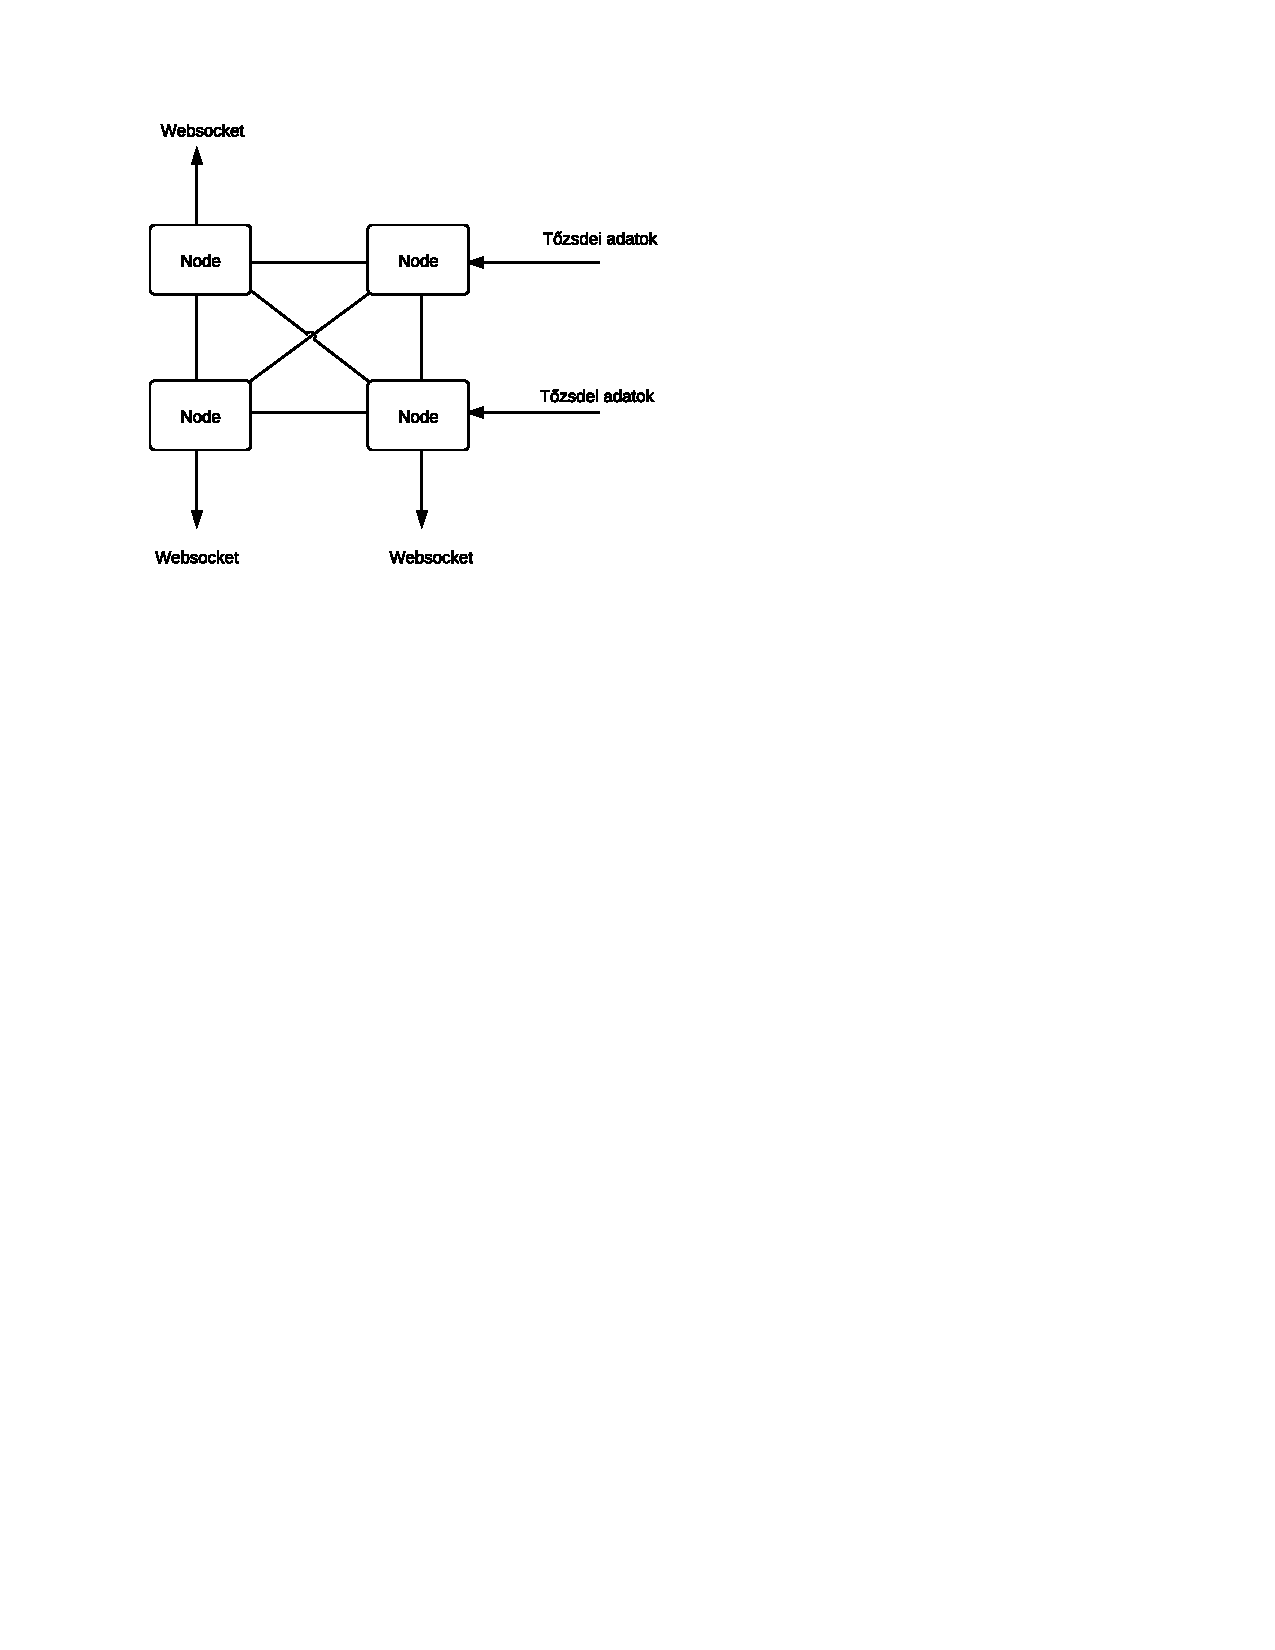
\includegraphics[clip=true, trim= 0 18cm 0 1cm]{fig/NodesWeb.pdf}
\end{figure}

A több node használata egyrészt redundanciát biztosít, másrészt nagyszámú
felhasználó esetén lehetőséget ad a terhelés megosztására. Ahhoz, hogy a
terhelésmegosztás egyszerű feladat legyen, a rendszer tervezésénél gondoskodni
kell arról, hogy két kérés-válasz (\emph{request-response}) forduló között ne
legyen semmilyen függőség (\emph{stateless}). Van olyan megoldás, hogy adott IP
címről érkező kéréseket mindig ugyanarra a gépre irányítja (\emph{sticky
session}, így csak egy gépen kell kezelni a felhasználó szerveroldali
,,állapotait''. Ez a megoldás esetünkben nem kielégítő, nem oldható meg a
szerverek közti egyenletes elosztás, ráadásul, ha a gép, amihez a felhasználó
éppen hozzá van rendelve, elromlik, a felhasználónak másik gépen újra be kell
lépnie stb.

A terhelésmegosztás nem része a rendszerünknek, azzal a feltételezéssel élünk,
hogy egy egyszerű \emph{DNS load balancer} végzi ezt a feladatot úgy, hogy
minden újabb kérést a soron következő node-nak továbbít (\emph{round robin}). 

Az ennek megfelelő felépítést REST architektúrának hívják. A REST:
\emph{Representational State Transfer}. A szerver a szolgáltatott
\emph{resource}-oknak különböző reprezentációit (\emph{representation})
küldi a kliensnek, a kérés tartalmaz minden információt, ami a válaszadáshoz
szükséges. A szerver nem tárol session-ben semmilyen állapotot a klienssel
kapcsolatban, így mindegy, hogy a soron következő kérések egyazon vagy más és
más szerverre érkeznek be \citep{Fielding}.

A HTTP protokoll \emph{szinkron protokoll}, a kliens által kezdeményezett
kapcsolaton keresztül kommunikál a szerver (választ ad), a szerver nem tud
kérés nélkül adatot küldeni a kliensnek \citep{HTTPSpec}. Ennek megoldására hozták (hozzák --
még folyamatban van a specifikálás) létre a HTTP protokollra épülő
\emph{websocket} protokollt\footnote{A websocket előtt is készült megoldás a
probléma áthidalására: a Comet. A dolgozat bemutató programjában a websocketre
egyszerűsége miatt esett a választás.}.  A websocket \emph{duplex protokoll},
mindkét irányba lehet adatot küldeni, ez lehetővé teszi, hogy a tőzsdei
információs alkalmazásunk a felhasználóknak azonnal kiküldje az adatokat
(\emph{push}), nem kell a böngészőnek időközönként lekérdeznie, van-e adat
(\emph{polling}) \citep{WebsocketSpec}.

A fenti ZM-től különválasztva, az önálló TL (TickerLine) alkalmazásban 
implementáljuk a websocket interfészt. A TL előfeltételei között szerepel, hogy
a ZM már fusson a node-on, hiszen a webalkalmazás mindössze annyiból áll, hogy
kapcsolatot biztosít a ZM és a böngésző között.

A példaprogramhoz a Cowboy HTTP szervert választottuk, mert a megismert OTP
könyvtárra épül, és tudja kezelni a websocket protokollt. A Cowboy saját
behaviour-t definiál: 

\begin{code}{erlang}{}
-module(tl_web_handler).
-behaviour(cowboy_http_handler).
-behaviour(cowboy_http_websocket_handler).
\end{code}

A behaviour-ök meghatározzák a callback függvényeket, amelyeket implementálni
kell. Esetünkben van egy \texttt{handle} függvény a HTTP request-ek
kezeléséhez, és van három websocket-et kezelő függvény, az
\texttt{websocket\_init}, a \texttt{websocket\_handle} és a
\texttt{websocket\_info}.

Induláskor, tehát akkor, amikor a kliens böngészője websocket kapcsolatot
kezdeményez, a process feliratkozik a \texttt{stock\_exchange} csatornára, 15
perces késleltetéssel (ennek mértékét lehetne például felhasználói előfizetés
alapján állítani).

\begin{code}{erlang}{}
websocket_init(_Any, Req, []) ->
  zm_channel:subscribe(stock_exchange, self(), [{delay, 15}]),
  Req2 = cowboy_http_req:compact(Req),
  {ok, Req2, undefined, hibernate}.
\end{code}

Amikor a kliens küld üzenetet a szervernek, akkor a process ezt a gen\_server
behaviour-höz hasonló módon kapja meg. A függvény visszatérési értékében
megadott választ megkapja a böngésző:

\begin{code}{erlang}{}
websocket_handle({text, Msg}, Req, State) ->
  {reply, {text, << "You said: ", Msg/binary >>}, 
           Req, State, hibernate};
\end{code}

A szerveren, a feliratkozás eredményeként érkező üzenetek továbbítása a
felhasználó felé:

\begin{code}{erlang}{}
websocket_info({msg, {_ChannelId, _SubscriptionRef}, 
               {Timestamp, {Share, Price,Count}}}, 
                Req, State) ->
  T = io_lib:format("~p: sold ~p pieces of ~p at \$~p",
                [calendar:now_to_local_time(Timestamp), 
                Count, Share, Price]),
  {reply, {text, list_to_binary(T)}, Req, State, hibernate};
\end{code}

Amikor a kliens zárja a kapcsolatot, a process leáll, és a
\texttt{zm\_sub\_mon} folyamat gondoskodik a leiratkozásról.

A szerver és a tőzsdei kereskedést adatait szimuláló process elindítása az
Erlang shell-ben. A véletlenszám generátorral készült adatokat 10
másodpercenként küldi a folyamat:

\begin{code}{erlang}{}
1> tl_app:start().
2> stock_exchange:start().
{ok,{interval,#Ref<0.0.0.22028>}}
\end{code}

A böngészőben az alábbi Javascript kód kezeli a websocket kapcsolatot:

\begin{code}{}{}
  if ("MozWebSocket" in window) {
    WebSocket = MozWebSocket;
  }
  if ("WebSocket" in window) {
    var ws = 
      new WebSocket("ws://tickerline.zakk.hu:9006/websocket");
    ws.onopen = function() {
      addStatus("Websocket connected.");
      ws.send("kakukk");
      addStatus("Testing connection...");
    };
    ws.onmessage = function (evt) {
      var msg = evt.data;
      addStatus("Received from server: " + msg);
    };
    ws.onclose = function() {
      addStatus("Websocket closed.");
    };
  } else {
    addStatus("Your browser does not support websockets.");
  }
\end{code}


\begin{figure}
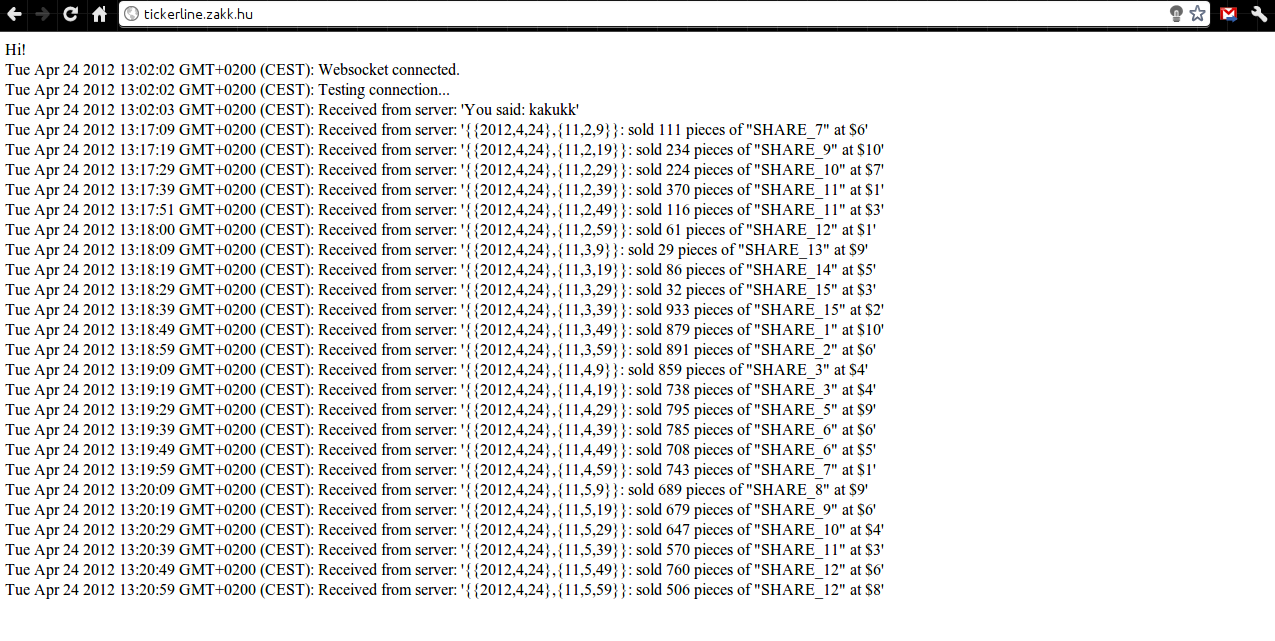
\includegraphics[scale=0.33]{fig/Browser.png}
\end{figure}

Ezzel elkészült a szerver, amely a tőzsdéről érkező kereskedési adatokat a
beállított késleltetéssel vagy real-time szolgáltatja a böngésző előtt
ülő fehasználóknak. A szerver redundánsan működik, ha valamelyik gép
meghibásodik, a következő kérés egy másikra fut be, és onnan kapja tovább az
adatokat (websocket esetében a fenti javascript \texttt{ws.onclose}
függvényéven lehet kezelni a kapcsolatban fellépő hibákat -- új kapcsolatot
létesíteni egy másik géppel).

Az alábbi képernyőképen látható az eredmény a böngészőben.

\chapter{Összegzés}
A dolgozatban végigvettük az Erlang nyelv alapjait, beleértve a szintaxist és
a fejlesztési alapelveket, különös tekintettel a párhuzamos programozás
mikéntjére. Az Erlang rendszerek magas rendelkezésre állása és skálázhatósága
ugyanarról a tőről fakad: az egymástól függetlenül működő process-ek
önállósága, a köztük lévő kommunikációt biztosító aszinkron üzenetküldési
metódus (aktor modell) a funkcionális programozási elvekkel együttesen teszik
lehetővé elosztott rendszerek fejlesztését. A nyelvet a kezdetektől fogva
folyamatos működést biztosító szoftverek készítéséhez fejlesztették, az Erlang 
magas szintű nyelvként biztosítja a fejlesztő számára az egyszerű megvalósítást. 
Az Erlang kiforrott, számtalan üzleti projektben használt szoftverkönyvtára, az Open
Telecom Platform (OTP), a leggyakoribb programozási mintákat valósítja
meg, és keretrendszert biztosít összetettebb, hibatűrő rendszerek építéséhez.
Állatorvosi lóként megvizsgáltunk egy egyszerű -- tőzsdei kereskedési adatokat
szolgáltató -- példaprogramot, amely az OTP infrastruktúrára épülve bizosítja a
redundáns és \emph{soft real-time} működést a weben. A felhasználó a websocket
protokoll segítségével \emph{azonnal} láthatja a böngészőjében a tőzsdéről érkező
adatokat. Az üzemeltető -- tegyük fel -- kis cégnek lehetősége van arra, hogy az
üzlet sikerével párhuzamosan növelje a szerver-klaszter kapacitását: egyszerűen
csak el kell indítani egy újabb node-ot, és azzal ,,megpingetni'' az egyik
tagját a hálózatának. Onnantól kezdve az új gép is teljes jogú taggá vált.

A cél elsősorban az Erlang alapvető tulajdonságainak bemutatása volt, nem
néztük meg részletesen a fejlesztéssel járó programozási gyakorlatot (pl. unit
tesztek írása, modulok megfelelő szervezése), programozási elveket. A
hibakezelésről volt szó: a mindig előforduló szoftverhibákat nem kell megpróbálni
a kódban észrevenni és kezelni (pl. a java try-catch szisztémája szerint),
hanem hagyni kell a hibás process-t leállni, és az őt monitorozó másik
folyamatra bízni a hiba kezelését (ha szükséges). Ez a megoldás átláthatóbb
és kevesebb kódot eredményez -- kevesebb kód, kevesebb hibalehetőség. A B.
függelékben néhány lista-függvénnyel ízelítőt adunk a rekurzív programozásból,
az imperatív programozás világában élő szoftverfejlesztőknek (és ez a nagyon
nagy többség) hasznos lehet egy rövidke kitekintés, van élet a C-n, Java-n
kívül is. A dolgozat -- szándékosan -- nem foglalkozik más nyelvekkel, de nem
állítja, hogy az Erlang lenne az egyedüli üdvözítő út. A más nyelvekkel való
összehasonlítás (a Scala-t kell itt megemlíteni) egy külön írás tárgya lehetne.

A dolgozat terjedelmi korlátai miatt nem tudtunk kitérni minden alkalmazási
lehetőségre. További vizsgálódás tárgya lehet a példaprogram világméretű
előfizetői kör kiszolgálására alkalmas változatának kifejlesztése, annak
bemutatása, hogyan lehet több ezer számítógépen rendszert működtetni. 
Visszautalva a CAP-elméletre: ilyen méretű rendszernél, ha tartani akarjuk a
megfelelő válaszidőt, az adat nem lesz minden időpillanatban konzisztens
(\emph{eventual consistency}). Ilyen nagy rendszernél a hálózati látencia, a
hálózati hibák kezelése, a keresett adat megtalálása (mely gépeken van a
százezerből) mind mind komoly feladatot jelent, amelyeket kezelni kell tudni.

További alkalmazási terület lehet az adat- vagy szövegbányászat
(például üzleti intelligencia rendszerekben). Egy egyedülálló gép kapacitásait
meghaladó adatmennyiség feldolgozásához biztosíthat platformot egy párhuzamosan
működő Erlang klaszter. Akár azért, mert a sok adat nem fér el egy helyen, akár
azért, mert az feldolgozás idejét kell belátható tartamúra rövidíteni. Ennek
megvalósításához akár a Google \emph{map-reduce} modelljét is lehet alkalmazni. A
feladat partícionálása (map), majd az eredmény \emph{key-value} párok
feldogozása (reduce) kézenfekvő feladat az Erlang process-intézményével.

Érdekes feladat lenne időigényes gazdasági, statisztikai számítások
megvalósítása például az egyetemi hálózaton. Minden egyes gépen el lehet
indítani egy Erlang node-ot, ami alapesetben nem végez semmilyen
feladatot, nem terheli észrevehetően a processzort; a hallgató a gép előtt ülve
észre sem veszi, hogy nem csak a passziánsz fut a gépen. Ezek a 
szerverek tetszés szerint munkára foghatók. Egy-egy, a standard üzenetküldési
rendszeren keresztül kapott modul végezhet valamilyen számítást, amíg másik
modult nem küld a működtető, vagy amíg el nem végzi a feladatát. Ha feladat
egyszerű, és egy függvényben leírható, akkor elég ezt a függvényt
felparaméterezve elküldeni a node-ra, majd begyűjteni az eredményt
(a \texttt{spawn} a hálózat tetszőleges node-jára működik). Ezzel a
módszerrel viszonylag egyszerűen ki lehet használni az egyetemi
hálózat gépeinek üres CPU ciklusait, egyetlen nagy klaszterént munkára fogva a
gépeket időigényes feladatok elvégzéséhez.

\appendix
\chapter{A példaprogram elérhetősége}
A példaprogram két Erlang alkalmazásból áll: az elosztott üzenetküldő
rendszerből (ZM) és az erre épülő webalkalmazásból (TL). Mindkét alkalmazás
megtalálható a dolgozathoz mellékelt CD-n, és a \emph{github.com}-on is.
\\
\\
\noindent ZM: \url{https://github.com/czinkos/zm}\\
TL: \url{https://github.com/czinkos/tl}
\\
\\
\noindent A programok indítása az alábbi paranccsal lehetséges (linux változat).

\begin{code}{}{}
\$ run_erl -daemon var/pipe var/log \
    "erl -pa cowboy/ebin -pa zm/ebin -pa tl/ebin \
     -mnesia dir '\"mnesia\"' -setcookie tl -sname tl"
\end{code}

A TL alkalmazáshoz le kell tölteni a Cowboy HTTP szervert:
\url{https://github.com/extend/cowboy}.


\chapter{Példák rekurzióra}
\begin{code}{erlang}{Visszaadja a lista n. elemét.}
nth(N, _) when N < 0; not(is_number(N)) ->
  {badArg, "N must be >= 0"};
nth(_, []) ->
  {badArg, "out of index"};
nth(0, [H|_]) ->
  H;
nth(N, [_H|T]) ->
  nth(N - 1, T).
\end{code}

\begin{code}{erlang}{Elem beszúrása rendezett listába.}
insert(I, []) ->
  [I];
insert(I, [H|T]) when I > H ->
  [H | insert(I, T)];
insert(I, [H|T]) ->
  [I, H|T].
\end{code}

\begin{code}{erlang}{Lista rendezése a beszúrás függvénnyel.}
insertion_sort([]) ->
  [];
insertion_sort([H]) ->
  [H];
insertion_sort([H|T]) ->
  insert(H, insertion_sort(T)).
\end{code}

\begin{code}{erlang}{Lista egy részét adja vissza.}
sublist([], _) ->
  [];
sublist(_, N) when N =< 0 ->
  [];
sublist([H|_], 1) ->
  [H];
sublist([H|T], N) ->
  [H | sublist(T, N -1)].
\end{code}

\begin{code}{erlang}{Adott intervallum egész számait adja vissza.}
seq(Low, High) when Low > High ->
  {error, "High must be larger than Low"};
seq(High, High) ->
  [High];
seq(Low, High) ->
  [Low| seq(Low + 1, High)].
\end{code}

\begin{code}{erlang}{Lista másik lista után fűzése.}
append(L1, L2) ->
  append(L1, L2, []).
append([],[], Res) -> reverse(Res);
append([], [H|T], Res) ->
  append([], T, [H|Res]);
append([H|T], L2, Res) ->
  append(T, L2, [H|Res]).
\end{code}

\begin{code}{erlang}{Lista visszafelé.}
reverse(L) ->
  reverse(L, []).
reverse([], Res) ->
  Res;
reverse([H|T], Res) ->
  reverse(T, [H | Res]).
\end{code}

\newpage
\begin{code}{erlang}{Egymásba ágyazott listák kisimítása.}
flatten(L) -> flatten(L, []).
flatten([], Res) -> Res;
flatten([H|T], Res) ->
  flatten(H, flatten(T, Res));
flatten(H, Res) ->
  [H|Res].
\end{code}

\begin{thebibliography}{9}

\harvarditem[Erlang documentáció]{}{2012}{ErlangDoc}
{\scshape Anonymous}, Erlang R15B01 dokumentáció (2011) Web:
\url{http://www.erlang.org}.

\harvarditem[Akamai felmérés]{}{2006}{AkamaiReport} 
{\scshape Anonymous}, Akamai felmérés (2006): \emph{Retail web site performance: Consumer Reaction to a Poor Online
Shopping Experience} Web:
\url{http://www.akamai.com/dl/reports/Site_Abandonment_Final_Report.pdf},
letöltés dátuma: 2012-04-02.

\harvarditem[Armstrong]{}{2003}{ArmstrongThesis}
{\scshape Armstrong, J.} (2003): \emph{Making reliable distributed systems in the presence of software errors}. PhD.
thesis, The Royal Institute of Technology Stockholm, Sweden. Web:
\url{http://www.erlang.org/download/armstrong_thesis_2003.pdf}, letöltés
dátuma: 2012-04-01.

\harvarditem[Armstrong]{}{2007}{ArmstrongBook}
{\scshape Armstrong, J.} (2007): \emph{Programming Erlang: Software for a Concurrent World}. The Pragmatic
Bookshelf, USA.

\harvarditem[Cesarini -- Thomson]{}{2009}{CesariniBook}
{\scshape Cesarini, F. -- Thomson, S.} (2009): \emph{Erlang programming}.
O'Reilly Media, USA.

\harvarditem[Fielding]{}{2001}{Fielding}
{\scshape Fielding, R.} (2001): \emph{Architectural Styles and the Design of Network-based Software
Architectures}. PhD. thesis, University of California, Irvine. Web:
\url{http://www.ics.uci.edu/~fielding/pubs/dissertation/fielding_dissertation.pdf}, letöltés dátuma: 2012-04-
01.

\harvarditem[Fielding ed.]{}{1999}{HTTPSpec}
{\scshape Fielding, R. ed.} (1999): \emph{Hypertext Transfer Protocol --
HTTP/1.1}. Web: \url{http://www.w3.org/Protocols/rfc2616/rfc2616.html},
letöltés ideje: 2012-04-23.

\harvarditem[Gilbert -- Lynch]{}{2003}{CAP}
{\scshape Gilbert, S. -- Lynch, N.} (2003): \emph{Brewer’s Conjecture and the
Feasibility of Consistent, Available, Partition-Tolerant Web Services}. Web:
\url{http://lpd.epfl.ch/sgilbert/pubs/BrewersConjecture-SigAct.pdf}, letöltés
ideje: 2012-04-23.

\harvarditem[Hewitt]{}{2011}{Hewitt}
{\scshape Hewitt, C.} (2011): \emph{Actor Model of Computation: Scalable Robust
Information Systems}. Web: \url{http://arxiv.org/pdf/1008.1459v23.pdf},
letöltés dátuma: 2012-04-24.

\harvarditem[Hickson ed]{}{2012}{WebsocketSpec}
{\scshape Hickson, I. ed.} (2012): \emph{The WebSocket API, Editor's Draft 17
April 2012}. Web: \url{http://www.w3.org/TR/websockets/}, letöltés ideje:
2012-04-21.

\harvarditem[Hudak]{}{1989}{Hudak}
{\scshape Hudak, P.} (1989): \emph{Conception, Evolution and Application of Functional
Programming Languages}. ACM Computing Surveys, Vol. 21, No. 3., September, p.
359-411.

\harvarditem[Logan et al.]{}{2011}{OTPInAction}
{\scshape Logan, M. -- Merritt, E. -- Carlsson, R.} (2011): \emph{Erlang and OTP in Action}.
Manning Publications, USA.

\end{thebibliography}

\clearpage
\addcontentsline{toc}{chapter}{Tárgymutató}
\printindex

\end{document}
